%--------------------------------------------------------------
% thesis.tex 
%--------------------------------------------------------------
% Corso di Laurea in Informatica 
% http://if.dsi.unifi.it/
% @Facolt\`a di Scienze Matematiche, Fisiche e Naturali
% @Universit\`a degli Studi di Firenze
%--------------------------------------------------------------
% - template for the main file of Informatica@Unifi Thesis 
% - based on Classic Thesis Style Copyright (C) 2008 
%   Andr\'e Miede http://www.miede.de   
%--------------------------------------------------------------
\documentclass[twoside,openright,titlepage,fleqn,
	headinclude,12pt,a4paper,BCOR5mm,footinclude]{scrbook}
%--------------------------------------------------------------
\newcommand{\myItalianTitle}{Titolo italiano\xspace}
\newcommand{\myEnglishTitle}{Titolo inglese\xspace}
% use the right myDegree option
\newcommand{\myDegree}{Corso di Laurea in Informatica\xspace}
%\newcommand{\myDegree}{
	%Corso di Laurea Specialistica in Scienze e Tecnologie 
	%dell'Informazione\xspace}
\newcommand{\myName}{Giuliano Gambacorta\xspace}
\newcommand{\myProf}{Paolo Frasconi\xspace}
\newcommand{\myOtherProf}{Correlatore\xspace}
\newcommand{\mySupervisor}{Nome Cognome\xspace}
\newcommand{\myFaculty}{
	Scuola di Scienze Matematiche, Fisiche e Naturali\xspace}
\newcommand{\myUni}{\protect{
	Università degli Studi di Firenze}\xspace}
\newcommand{\myLocation}{Firenze\xspace}
\newcommand{\myTime}{Anno Accademico 2017-2018\xspace}
\newcommand{\myVersion}{Version 0.1\xspace}
%--------------------------------------------------------------
\usepackage[italian]{babel}
\usepackage[utf8x]{inputenc} 
\usepackage[T1]{fontenc} 
\usepackage[square,numbers]{natbib} 
\usepackage[fleqn]{amsmath}  
\usepackage{ellipsis}
\usepackage{listings}
\usepackage{subfig}
\usepackage{caption}
\usepackage{appendix}
\usepackage{siunitx}
\usepackage[pdftex]{graphicx}
%--------------------------------------------------------------
\usepackage{dia-classicthesis-ldpkg}
%--------------------------------------------------------------
% Options for classicthesis.sty:
% tocaligned eulerchapternumbers drafting linedheaders 
% listsseparated subfig nochapters beramono eulermath parts 
% minionpro pdfspacing
\usepackage[eulerchapternumbers,linedheaders,subfig,beramono,eulermath,
parts]{classicthesis}
%--------------------------------------------------------------
\newlength{\abcd} % for ab..z string length calculation
% how all the floats will be aligned
\newcommand{\myfloatalign}{\centering} 
\setlength{\extrarowheight}{3pt} % increase table row height
\captionsetup{format=hang,font=small}
%--------------------------------------------------------------
% Layout setting
%--------------------------------------------------------------
\usepackage{geometry}
\geometry{
	a4paper,
	ignoremp,
	bindingoffset = 1cm, 
	textwidth     = 13.5cm,
	textheight    = 21.5cm,
	lmargin       = 3.5cm, % left margin
	tmargin       = 4cm    % top margin 
}

\lstset{
  	frame=tb,
	language=Matlab,
  	aboveskip=3mm,
  	belowskip=3mm,
  	showstringspaces=false,B
  	columns=flexible,
  	basicstyle={\small\ttfamily},
  	numbers=none,
  	breaklines=true,
  	breakatwhitespace=true,
  	tabsize=3
}
%--------------------------------------------------------------
\begin{document}
\frenchspacing
\raggedbottom
\pagenumbering{roman}
\pagestyle{plain}
%--------------------------------------------------------------
% Frontmatter
%--------------------------------------------------------------
%--------------------------------------------------------------
% titlepage.tex (use thesis.tex as main file)
%--------------------------------------------------------------
\begin{titlepage}
	\begin{center}
   	\large
      \hfill
      \vfill
      \begingroup
         
\includegraphics[scale=0.15]{logo/LOGO}\\
%			\spacedallcaps{\myUni} \\ 
			\myFaculty \\
			\myDegree \\ 
			\vspace{0.5cm}
         \vspace{0.5cm}    
         Tesi di Laurea    
      \endgroup 
      \vfill 
      \begingroup
      	\color{Maroon}\spacedallcaps{\myItalianTitle} \\ $\ $\\
      	\spacedallcaps{\myEnglishTitle} \\ 	
	\bigskip
      \endgroup
      \spacedlowsmallcaps{\myName}
      \vfill 
      \vfill
      Relatore: \emph{Paolo Frasconi}\\
      % Correlatore: \emph{Correlatore}\\
      \vfill
      \vfill
      \myTime
      \vfill                      
	\end{center}        
\end{titlepage}   
%--------------------------------------------------------------
% back titlepage
%--------------------------------------------------------------
   \newpage
	\thispagestyle{empty}
	\hfill
	\vfill
	\noindent\myName: 
	\textit{\myItalianTitle,} 
	\myDegree, \textcopyright\ \myTime
%--------------------------------------------------------------
% back titlepage end
%--------------------------------------------------------------
\pagestyle{scrheadings}
%--------------------------------------------------------------
% Mainmatter
%--------------------------------------------------------------
\pagenumbering{arabic}
% use \cleardoublepage here to avoid problems with pdfbookmark
%\include{intro} % use \myChapter command instead of \chapter
\tableofcontents
\listoffigures
\cleardoublepage
\thispagestyle{empty}
\begin{flushright}
\null\vspace{\stretch {1}}
\emph{"citazione" \break --- Autore} \vspace{\stretch{2}}\null
\end{flushright}
\cleardoublepage
\myChapter{Introduzione}
\section{Prefazione}
\label{sec:prefazione}
Lo scopo di questo elaborato è la riproduzione e lo studio di \textit{sketch-rnn} \cite{sketchrnn}: un modello generativo in grado di produrre schizzi di semplici oggetti, composti da sequenze di tratti, appresi da un dataset di disegni creati da esseri umani. Il dataset è costantemente ampliato tramite \textit{Quick Draw!} \cite{quickdraw}, un gioco online in cui agli utenti viene chiesto di riprodurre alcuni oggetti entro 20 secondi, che al momento attuale costituisce la più vasta collezione di disegni al mondo. In questo lavoro viene proposto un prototipo in \textit{Keras} \cite{keras}, un framework che a sua volta poggia su \textit{tensorflow} \cite{tensorflow}, che è la libreria software utilizzata per il lavoro originale.
\begin{figure}[ht]
	\centering
	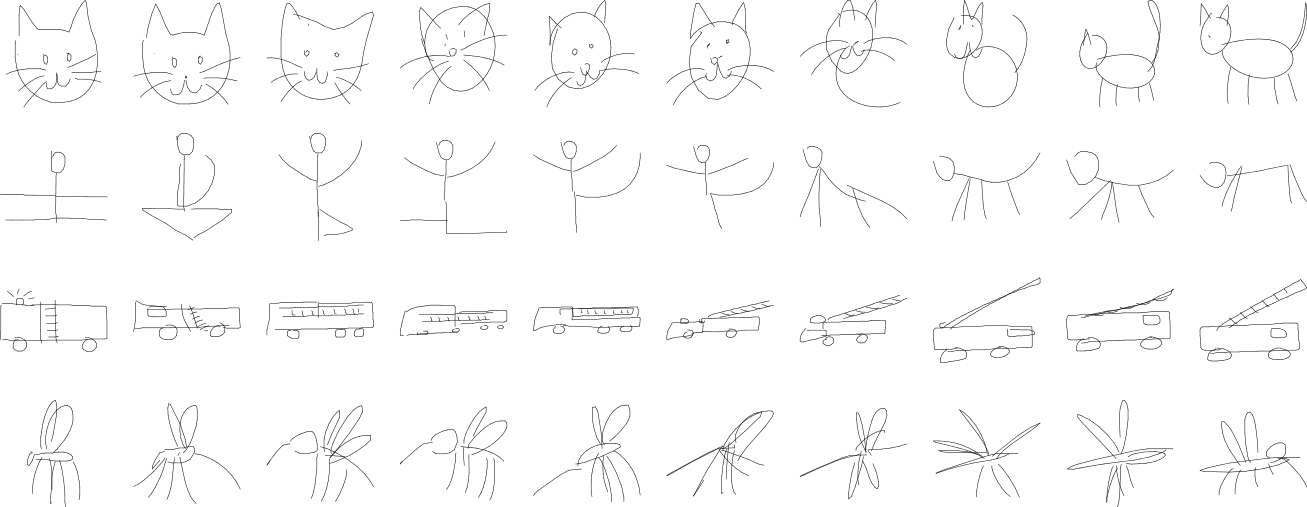
\includegraphics[width=\linewidth]{img/sketch_rnn_latent.png}
	\caption{Interpolazioni nello spazio di latenza di immagini vettoriali generate dal modello.}
	\label{fig:1.1}
\end{figure}
\section{Stato dell'arte}
Negli ultimi anni la generazione di immagini attraverso l'uso di reti neurali ha avuto ampia diffusione, fra i modelli più importanti possiamo citare: \textit{Generative Adversarial Networks (GANs)} \cite{GAN}, \textit{Variational Inference (VI)} \cite{VI} e \textit{Autoregressive Density Estimation (AR)} \cite{AR}. Il limite della maggior parte di questi algoritmi consiste nel fatto che lavorano con figure in pixel a bassa risoluzione, a differenza degli animali complessi che, piuttosto che vedere il mondo come una griglia di pixel, astraggono concetti per rappresentare ciò che osservano. Allo stesso modo degli esseri umani, che fin da piccoli imparano a riportare le proprie idee attraverso una sequenza di tratti su un foglio, questo modello generativo apprende da, e produce, immagini vettoriali.

L'obbiettivo è di addestrare una macchina a riprodurre ed astrarre concetti, in maniera analoga a come farebbe una persona. Ciò può avere numerose applicazioni in campo didattico come artistico, ad esempio assistendo il processo creativo, così come l'analisi della rappresentazione prodotta può offrire spunti di ricerca.
\section{Reti neurali}
Per spiegare le reti neurali e il Deep Learning si possono usare diversi approcci: si può ad esempio seguire il corso storico, introducendo il concetto di \textit{Percettrone}, passando ai Percettroni Multi-Strato ed ai primi metodi di ottimizzazione che furono applicati a questi modelli. Un'altra possibilità consiste nel partire da un punto di vista stocastico, definendo una regressione logistica che implica in modo naturale la minimizzazione di una \textit{loss function}. Ciò permette di definire il concetto stesso di loss function e il principio secondo cui modificare dei parametri per ottenere una soluzione migliore, il che si ricollega perfettamente al concetto di Percettrone Multi-Strato come classificatore di una regressione logistica.

Di seguito verrà proposta la spiegazione di alcuni modelli fondamentali del Deep Learning, che saranno considerati come "mattoni" costitutivi della rete neurale studiata in questo progetto. Ciò aiuterà a comprendere agevolmente l'implementazione realizzata nel codice, seguendo un punto di vista coerente con le piattaforme più diffuse.
\section{Reti densamente connesse} % (fold)
\label{sec:reti_densamente_connesse}
Un neurone artificiale consiste in una funzione matematica che costituisce l'unità computazionale di base di una rete neurale artificiale.
\begin{figure}[ht]
	\centering
	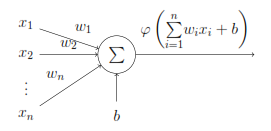
\includegraphics{img/artificial_neuron.PNG}
	\caption{Rappresentazione di un neurone artificiale.}
	\label{fig:1.2}
\end{figure}

Come si nota dalla figura \ref{fig:1.2} il neurone artificiale riceve \emph{n} input pesati $(w_1x_1,...,w_nx_n)$ e un bias \emph{b}. Successivamente li somma e applica una funzione non lineare nota come \textit{activation function} $\varphi$ per generare l'output. In sostanza calcolare l'output di un singolo neurone corrisponde a formare una combinazione lineare dei suoi input pesati e poi passarla ad una funzione di attivazione.

Per ragioni storiche, nel caso particolare in cui la funzione di attivazione consista di una funzione con una soglia lineare (e output binario), il neurone è detto \textit{Percettrone}.

Da qui in poi, quando ci riferiremo ad un \textit{layer} (strato) di una rete neurale staremo parlando di un raggruppamento di neuroni che formano, nello specifico, una colonna nel grafo della figura \ref{fig:1.2}, ovvero neuroni che si trovano allo stesso livello di profondità nella rete. Inoltre, ogni layer che si trova fra quello di input e quello di output verrà chiamato \textit{hidden layer}.

Come detto in precedenza, un Percettrone Multi-Strato (MLP da Multi-Layer Perceptron) può essere visto come un classificatore a regressione logistica dove l'input è manipolato utilizzando una trasformazione non lineare appresa $h(\boldsymbol{x})$ che costituisce l'hidden layer della nostra rete neurale (come in figura \ref{fig:1.2}). Questa operazione proietta l'input in uno spazio in cui diventa linearmente separabile.

Questa computazione eseguita da una rete neurale multi-Strato, con un singolo hidden layer con una funzione di attivazione non lineare per elementi $\varphi_i$ che proietta il vettore di input \textbf{x} verso l'hidden output, può essere scritta in forma matriciale come $\boldsymbol{y} = \varphi_2(W_2\varphi_1(W_1\boldsymbol{x} + \boldsymbol{b_1}) + \boldsymbol{b_2})$ dove $W_i, \boldsymbol{b_i}$ sono la matrice dei pesi e il vettore del bias dell'\textit{i}-esimo layer.

\begin{figure}[ht]
	\centering
	\begin{tikzpicture}[shorten >=1pt,->,draw=black!50, node distance=\layersep]
	    \tikzstyle{every pin edge}=[<-,shorten <=1pt]
	    \tikzstyle{neuron}=[circle,fill=black!25,minimum size=17pt,inner sep=0pt]
	    \tikzstyle{input neuron}=[neuron, fill=green!50];
	    \tikzstyle{output neuron}=[neuron, fill=red!50];
	    \tikzstyle{hidden neuron}=[neuron, fill=blue!50];
	    \tikzstyle{annot} = [text width=4em, text centered]

	    % Draw the input layer nodes
	    \foreach \name / \y in {1,...,3}
	    % This is the same as writing \foreach \name / \y in {1/1,2/2,3/3,4/4}
	        \node[input neuron, pin=left:Input \#\y] (I-\name) at (0,-\y) {};

	    \node[input neuron, pin=left:Input \#n] (I-4) at (0,-5) {};

	    % Draw the hidden layer nodes
	    \foreach \name / \y in {1,...,4}
	        \path[yshift=0.5cm]
	            node[hidden neuron] (H-\name) at (\layersep,-\y cm) {};

	    \node[hidden neuron] (H-5) at (\layersep,-5.5 cm) {};

	    % Draw the output layer node
	    \node[output neuron,pin={[pin edge={->}]right:Output}, right of=H-3] (O) {};

	    % Connect every node in the input layer with every node in the
	    % hidden layer.
	    \foreach \source in {1,...,4}
	        \foreach \dest in {1,...,5}
	            \path (I-\source) edge (H-\dest);

	    % Connect every node in the hidden layer with the output layer
	    \foreach \source in {1,...,5}
	        \path (H-\source) edge (O);

	    % Annotate the layers
	    \node[annot,above of=H-1, node distance=1cm] (hl) {Hidden layer};
	    \node[annot,left of=hl] {Input layer};
	    \node[annot,right of=hl] {Output layer};
	\end{tikzpicture}
	\caption{Rappresentazione di un modello Multi-Strato.}
	\label{fig:1.3}
\end{figure}

% \begin{figure}[ht]
% 	\centering
% 	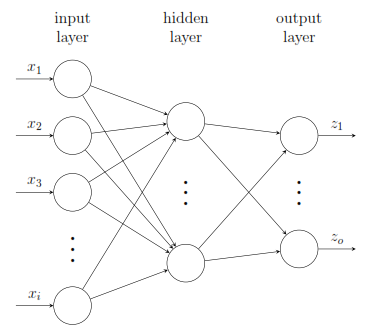
\includegraphics{img/MLN.png}
% 	\label{fig:1.3}
% \end{figure}

Seguendo il teorema di approssimazione universale \cite{approx} possiamo affermare che una rete neurale con un singolo hidden layer contenente un numero finito di neuroni (ovvero un MLP) è sufficiente per approssimare qualunque funzione continua su un sottoinsieme compatto di $\mathbb{R}^n$.

Alcuni sinonimi rilevanti utilizzati al posto di reti neurali Multi-Strato 
sono \textit{dense layers}, \textit{fully-connected layers} o, meno diffuso, \textit{inner product layers}.
% section reti_densamente_connesse (end)
\section{Reti ricorrenti}
\label{sec:reti_ricorrenti}
\begin{figure}[ht]
	\centering
	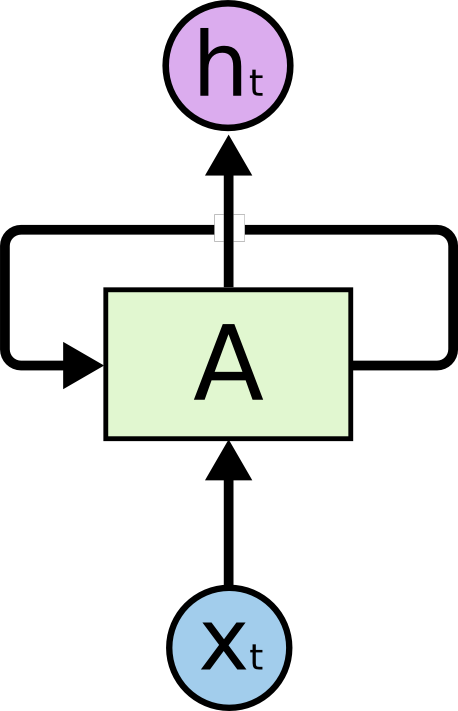
\includegraphics{img/RNN.png}
	\caption{Una semplice RNN (Recurrent Neural Network).}
	\label{fig:1.4}
\end{figure}
Il cervello umano, nello specifico il lobo frontale, è in grado di elaborare conseguenze future risultanti da azioni nel presente, ha inoltre la capacità di selezionare fra buone e cattive azioni (o fra migliori e ideali) e può determinare somiglianze e differenze fra oggetti ed eventi.

Molti problemi per essere risolti necessitano di un certo grado di conoscenza pregressa. Un esempio può riguardare le variazioni della luce di un semaforo: se, per esempio, si osserva che in un dato istante la luce accesa è quella gialla, lo scopo sarebbe quello di sapere quale sarà la prossima ad accendersi. Le diverse posizioni delle luci in un semaforo sono irrilevanti: ciò che interessa sapere è quale colore apparirà, sapendo che quello appena apparso è il giallo. Nella maggior parte delle città è noto che la risposta sarebbe il rosso. Per rispondere a questa domanda è venuta in aiuto l'esperienza ma se si provasse a risolvere il problema utilizzando una rete neurale come quella proposta in precedenza non si otterrebbe una risposta soddisfacente. Ciò accade perché risolvere il problema comporta di considerare una dipendenza temporale, che corrisponde al metodo attraverso cui un essere umano impara a risolvere problemi: analizzando sequenze di eventi.

Per trovare una soluzione a questo problema, com'è uso nel campo dell'Intelligenza Artificiale, si parte ancora una volta dai modelli basati sui principi biologici per elaborare una classe di reti neurali artificiali, in cui le connessioni fra le unità formano un ciclo orientato, dette Reti Neurali Ricorrenti (RNN da Recurrent Neural Networks, Fig. \ref{fig:1.4}). Queste connessioni creano uno stato interno della rete che le permette di esibire un comportamento dinamico nel tempo.

Per quanto riguarda le reti neurali non ricorrenti sono già state presentate molte conoscenze utili allo scopo di ottenere buoni parametri, di conseguenza si rende necessario trovare un modo di trasferire le potenzialità già discusse anche su questo nuovo tipo di reti neurali. Un'idea primitiva sarebbe quella di elaborare la rete ricorrente attraverso copie molteplici di una singola rete, come si vede in fig. \ref{fig:1.5}, trasferendo le informazioni dall'hidden layer \textit{A} alla copia successiva per realizzare una forma di memorizzazione.

\begin{figure}[ht]
	\centering
	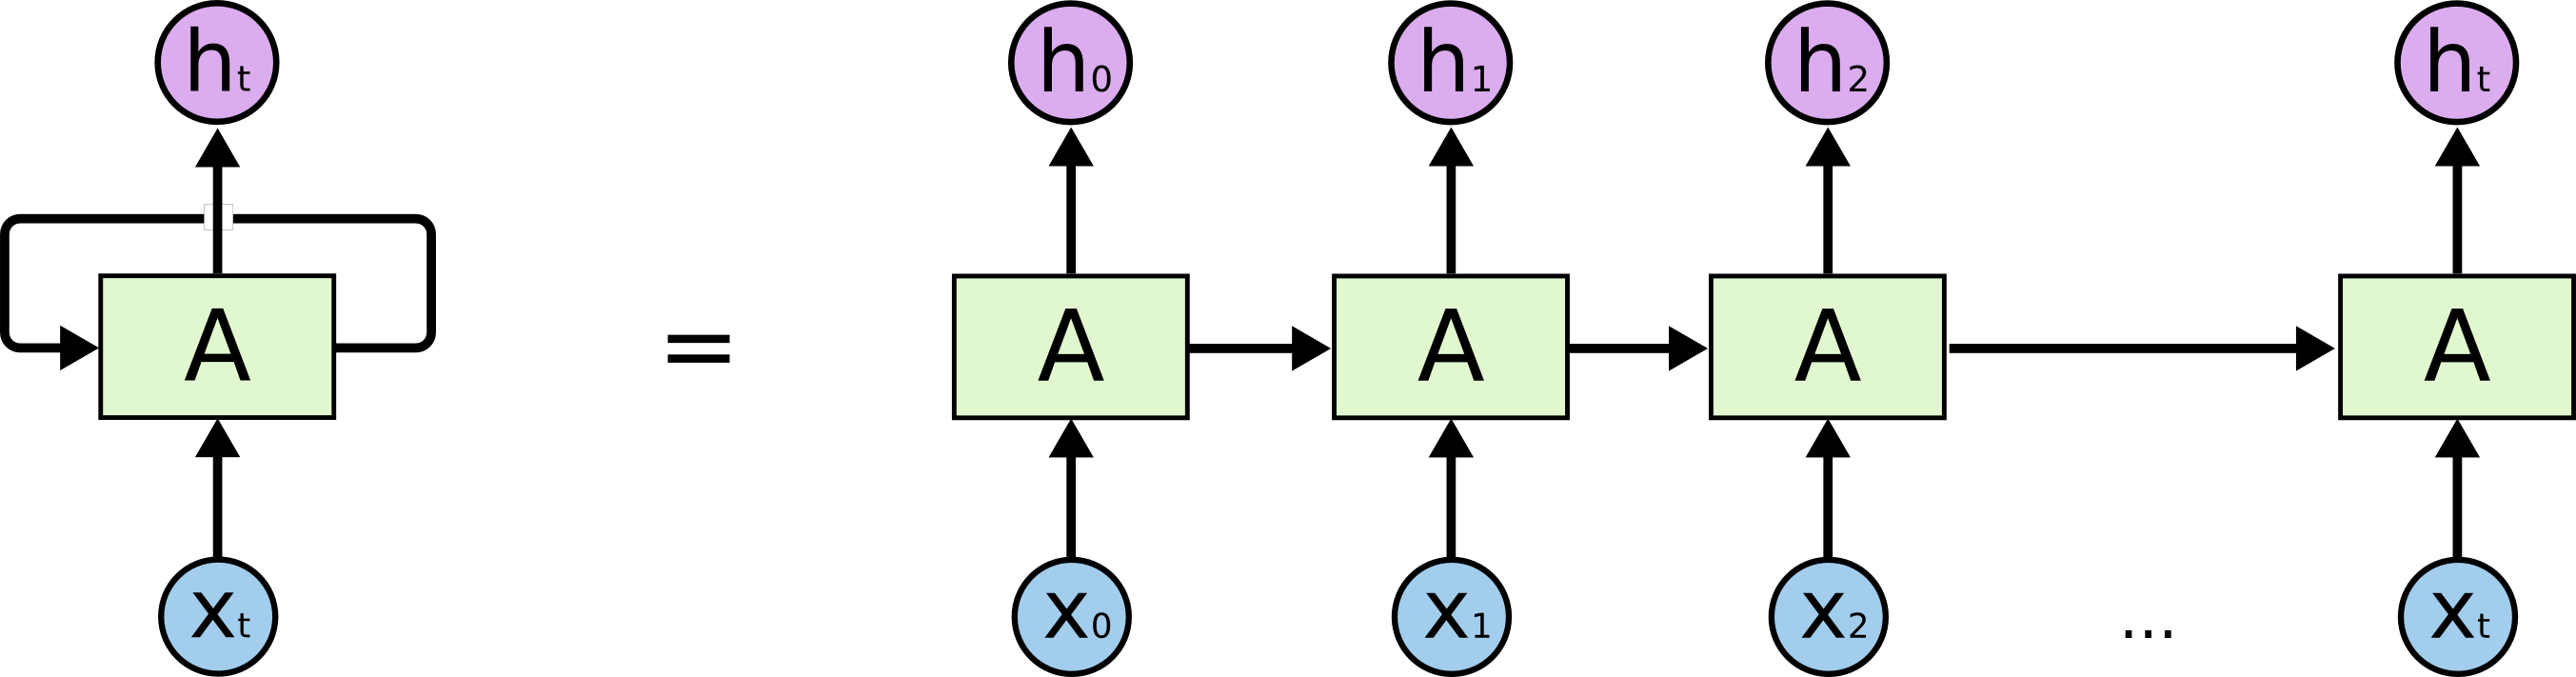
\includegraphics{img/unrolled_rnn.png}
	\caption{Una RNN dispiegata lungo la linea temporale.}
	\label{fig:1.5}
\end{figure}

Tuttavia ci potrebbero essere diversi modi di intendere la memoria e di combinare l'input del \textit{time-step} attuale con le informazioni ottenute dal precedente. Si prendano in considerazione due esempi: nel primo si sceglie di ottenere le informazioni precedenti conservando l'input, nel secondo l'hidden layer del time-step passato, ottenendo risultati completamente diversi. in fig. \ref{fig:1.6} sono riportati i due esempi sopra descritti, dove ogni colore rappresenta gli effetti sulla memoria dell'hidden layer \textit{A}.
\begin{figure}[ht]
	\centering
	\begin{tabular}{cc}
		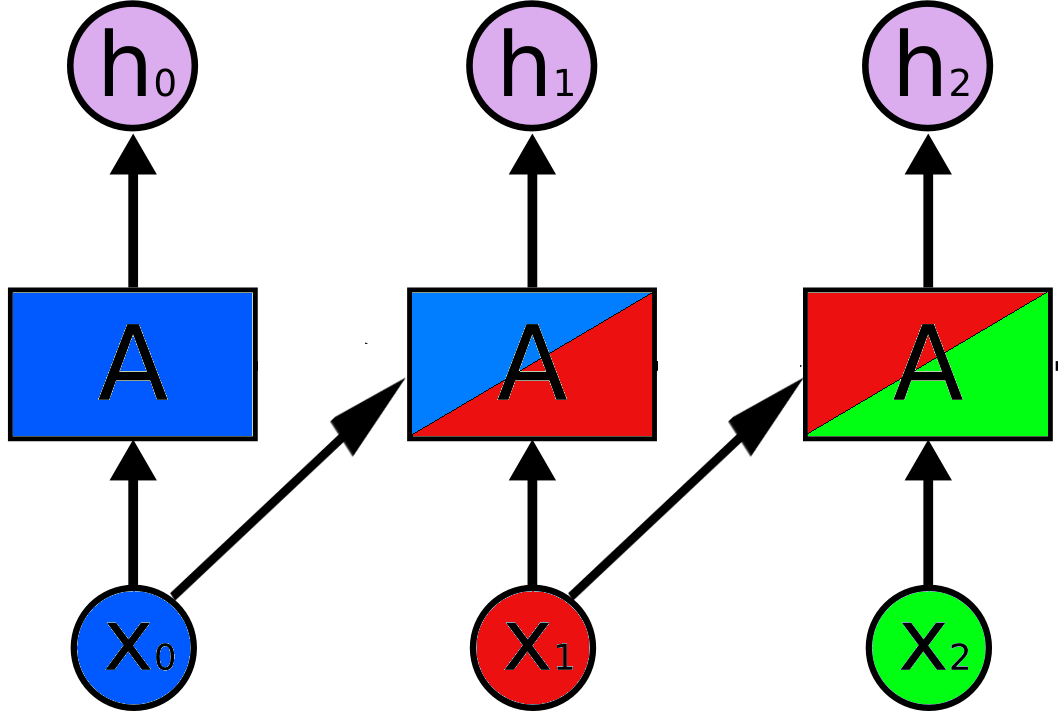
\includegraphics[width=0.4\linewidth]{img/input_memory.png} &
		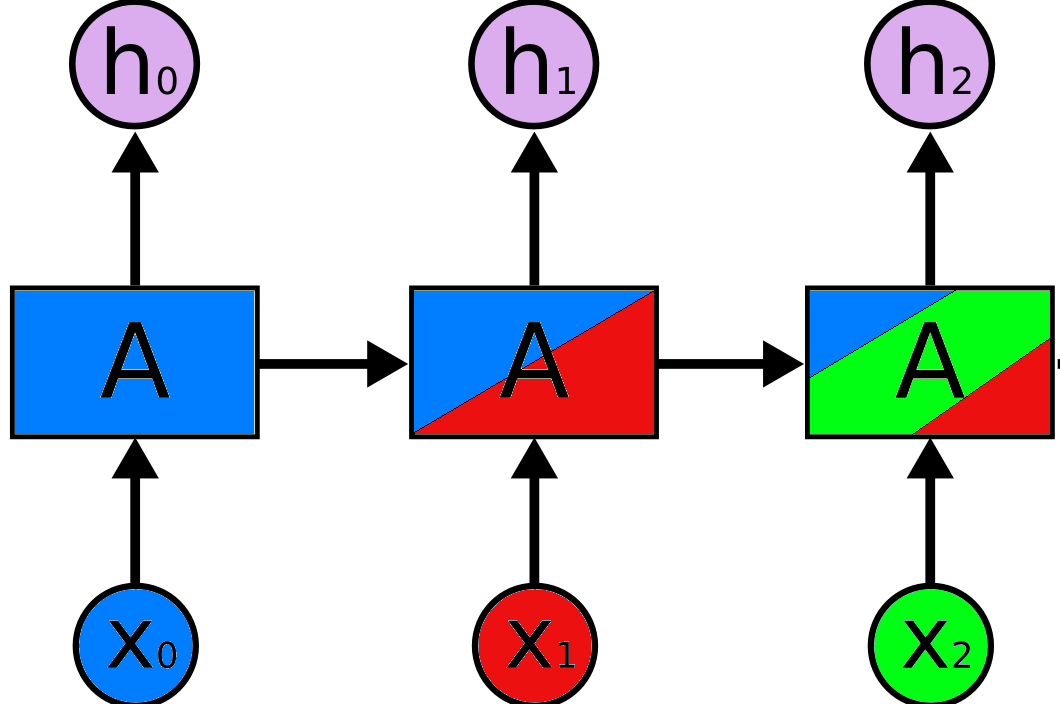
\includegraphics[width=0.4\linewidth]{img/hidden_memory.png} \\
		\footnotesize (a) Visualizzazione della memoria usando & \footnotesize (b) Visualizzazione della memoria usando \\ \footnotesize la ricorrenza dell'input & \footnotesize la ricorrenza dell'hidden layer
	\end{tabular}
	\caption{Due diversi metodi di implementazione della memoria in una RNN}
	\label{fig:1.6}
\end{figure}

Come si può vedere in fig. \hyperref[fig:1.6]{6(a)}, usando la ricorrenza dell'input viene memorizzato solo l'attuale input e il precedente, invece nel caso della ricorrenza dell'hidden layer (fig. \hyperref[fig:1.6]{6(b)}) viene ricordata una mistura di tutti gli input precedenti. Per comprendere perché la seconda ipotesi è migliore si può usare questo esempio: si immagini di voler dedurre la parola seguente a \textit{"I love"} ("io amo") e che il testo contenga le affermazioni \textit{"I love you"} ("ti amo") e \textit{"I love carrots"} ("amo le carote"). Se lo scopo è predire la decisione che verrà presa fra queste due opzioni e non sono note altre informazioni al di là dell'input (nel caso della ricorrenza dell'input), la rete neurale non avrà abbastanza informazioni per decidere. Viceversa, se la rete neurale possiede informazioni riguardanti il contesto, ad esempio se precedentemente si è parlato di cibo o di pasti, la sceltà diventerà più chiara. In teoria la ricorrenza dell'hidden layer può essere interpretata come un tentativo di ricordare ogni informazione con cui la rete neurale è entrata in contatto, ma in pratica vige un limite tutt'al più di qualche passo.

Un'altra caratteristica delle RNN, che le avvantaggia ulteriormente rispetto alle MLN, è la versatilità. Le RNN, infatti, sono in grado di operare su sequenze di vettori, a differenza delle MLN o delle CNN (che non saranno trattate in questo elaborato) che operano su vettori di dimensioni fissate, così come fissato è il numero di passi computazionali (limitato ad esempio dal numero di hidden layers). Si possono elaborare sequenze sia in input che in output (o entrambi), in fig. \ref{fig:1.7} si distinguono cinque casi.
\newpage
\begin{figure}[ht]
	\centering
	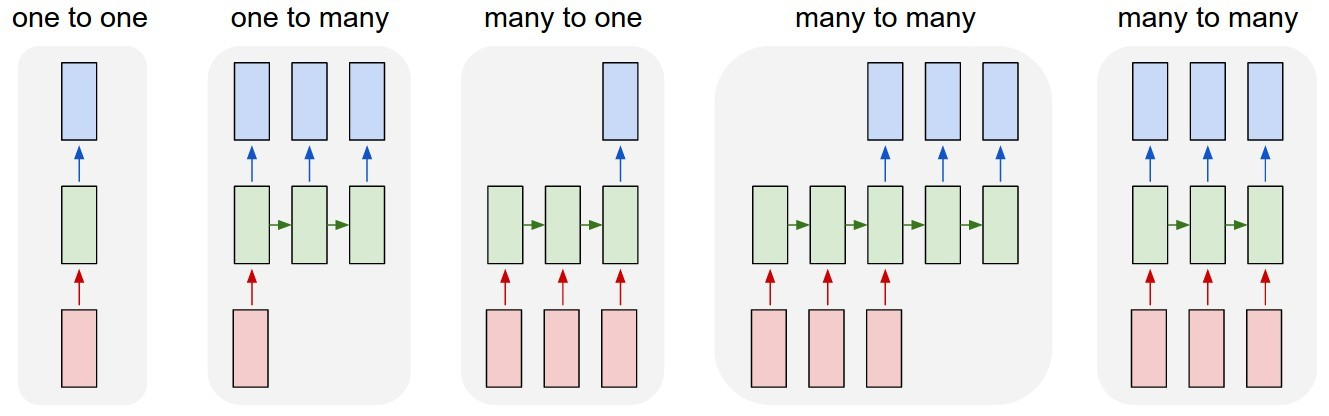
\includegraphics{img/rnn_seq.jpg}
	\caption{Combinazioni di sequenze vettoriali. \cite{rnn_effect}}
	\label{fig:1.7}
\end{figure}

\begin{enumerate}
	\label{enum:recurrence}
	\item[Uno a uno:] il caso più semplice, in cui non vi è ricorrenza, ad esempio nella classificazione di immagini.
	\item[Uno a molti:] il caso in cui è presente una sequenza in output. Tipicamente usato nella creazione di sottotitoli, dove ad una sola immagine corrisponde una frase.
	\item[Molti ad uno:] in questo caso la sequenza è presente solo in input, è la struttura della \textit{sentiment analysis}, dove da una frase viene estratta la sensazione positiva/negativa contenuta in essa.
	\item[Molti a molti:] qui abbiamo una sequenza sia in input che in output, si potrebbe trattare di un modello di traduzione che assegna ad una frase in una lingua la frase corrispondente in un'altra.
	\item[Molti a molti (sinc.):] come nell'esempio precedente, ma l'output è in sincronia con l'input. Utilizzato ad esempio nella classificazione video, in cui un'etichetta va assegnata ad ogni frame in tempo reale.
\end{enumerate}
\subsection{Dipendenze a lungo termine} % (fold)
\label{sub:dipendenze_a_lungo_termine}
\begin{figure}[ht]
	\centering
	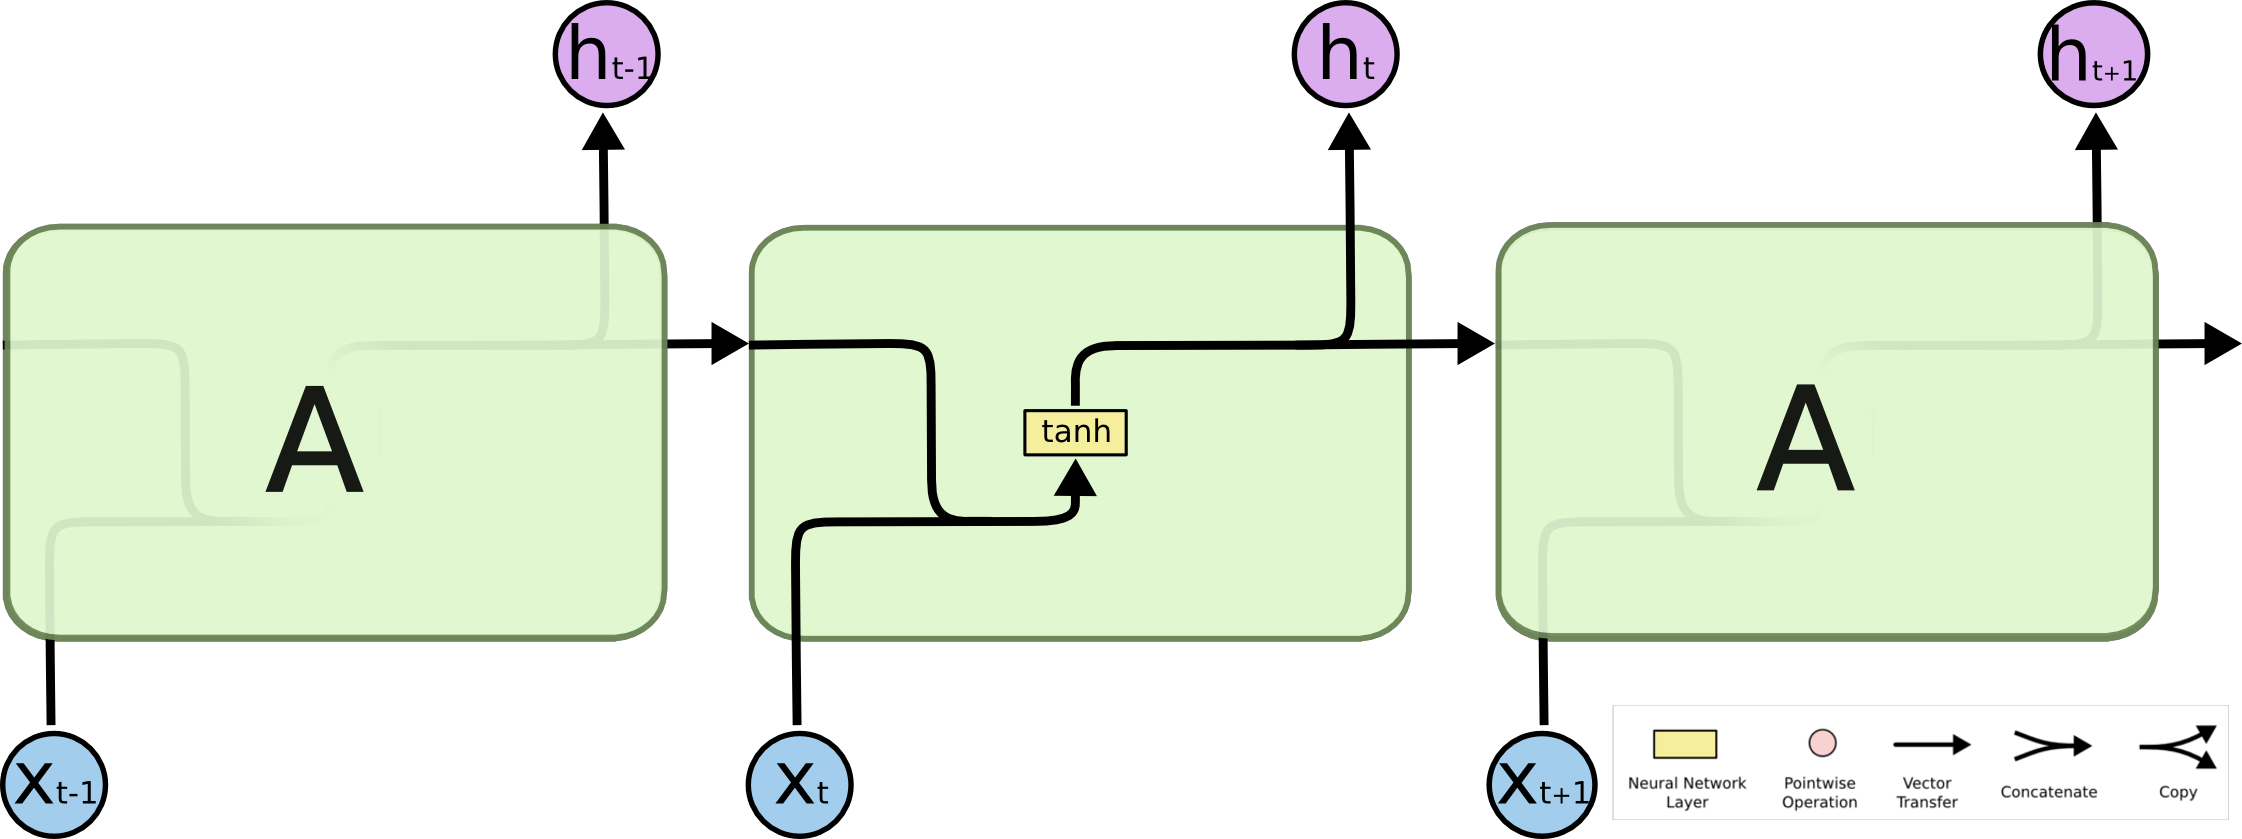
\includegraphics{img/rnn_struct.png}
	\caption{Struttura interna di una RNN standard con un singolo hidden layer.}
	\label{fig:1.8}
\end{figure}
Nel progettare una RNN va presa in considerazione la possibilità di trovarsi nella condizione di dover fornire un vasto numero di informazioni dal contesto per risolvere un problema. Tornando al compito della previsione di parole in un testo, si supponga di dover completare la frase "sto per andare a nuotare in", le informazioni a breve termine suggeriscono che la parola successiva sia un luogo dove sia possibile nuotare e sapendo che la frase precedente è "la spiaggia è molto assolata" si potrebbe dedurre che la parola da predire sia "mare". Il problema in questione è che si incontrano spesso difficoltà nell'identificare informazioni rilevanti. La formulazione di RNN data finora, in teoria, è perfettamente in grado di gestire dipendenze a lungo termine. In pratica, come spesso accade, si tratta di una prova tipicamente banale per una mente umana ma che una semplice implementazione (come in fig. \ref{fig:1.8}) non sarebbe in grado di risolvere efficacemente. Uno degli ostacoli più frequenti da risolvere è il cosiddetto problema del gradiente evanescente (\textit{vanishing gradient} \cite{vanishing}), per superarlo si rendono necessarie varianti più elaborate della RNN semplice, come le LSTM.
% subsection dipendenze_a_lungo_termine (end)
\subsection{Long Short Term Memory}
\label{sub:lstm}
\begin{figure}[ht]
	\centering
	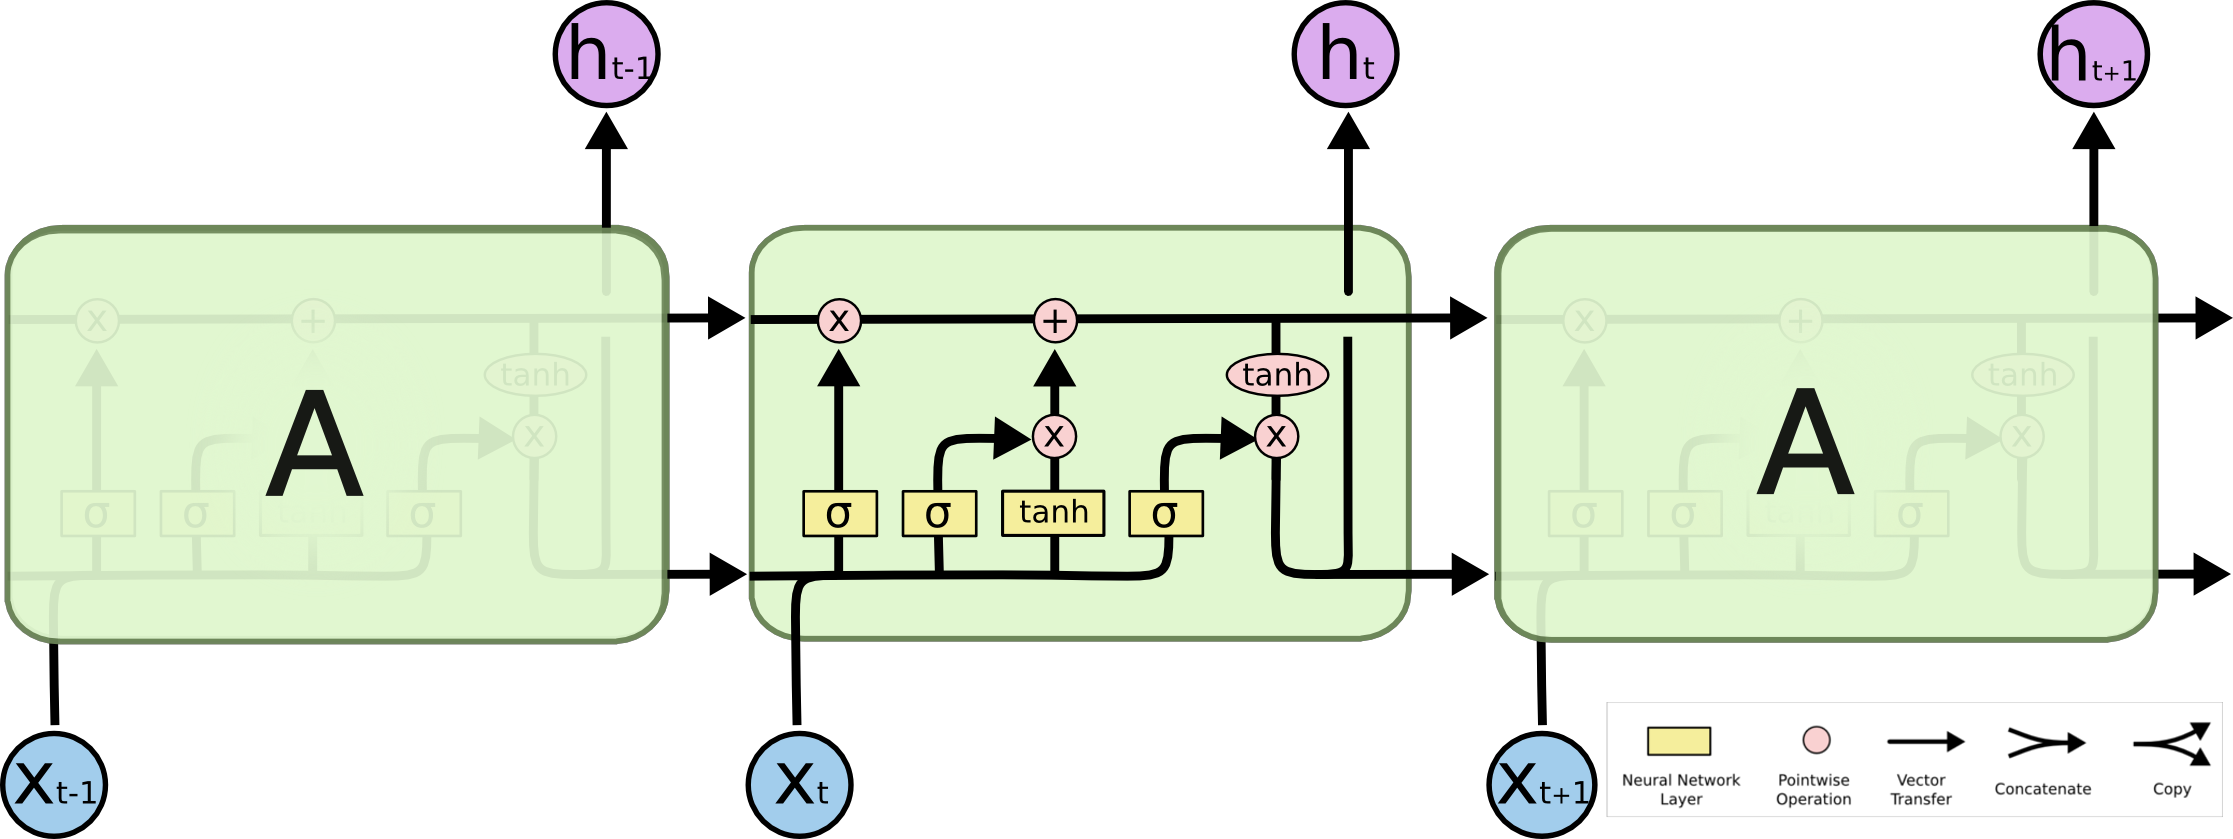
\includegraphics{img/lstm_struct.png}
	\caption{Struttura interna di una lstm che evidenzia i quattro strati interni di un layer. Immagine da \cite{LSTM}}
	\label{fig:1.9}
\end{figure}
Per ottenere una RNN in grado di apprendere dipendenze a lungo termine, Hochreiter and Schmidhuber \cite{vanishing} introdussero, nel 1997, una versione detta \textit{Long Short Term Memory (LSTM)}.

A differenza di una RNN standard, che si limita ad una semplice struttura ripetuta, le LSTM operano una computazione complessa per ottenere lo stato interno. Invece della sola funzione di attivazione, una LSTM possiede strumenti per rimuovere, aggiungere o lasciar passare intatta l'informazione attraverso lo stato corrente del layer, detti \textit{gates} (cancelli). Questi gates sono composti da layer con attivazione sigmoide e operazioni di somma o moltiplicazione punto a punto, che definiscono quanto lasciar passare di ogni componente in ingresso.

Seguendo il diagramma in fig. \ref{fig:1.9}, vediamo in basso a sinistra il primo layer sigmoide, detto \textit{forget gate layer}, che si occupa di decidere quale informazione scartare dallo strato precedente o dall'input. Successivamente abbiamo il secondo layer sigmoide, detto \textit{input gate layer}, che decide quali valori saranno aggiornati, tramite l'output di un layer a tangente iperbolica. Questa combinazione va a modificare lo stato interno della LSTM, il quale attraversa la linea orizzontale superiore, che verrà poi trasferito allo stato successivo. Infine, dopo aver attraversato un'altra tangente iperbolica (per standardizzare i valori fra -1 e 1), un'altra sigmoide opera da gate per regolare l'output. \footnote{Esiste un'ampia varietà di modelli basati sulle LSTM, si suggeriscono: LSTM con "peephole connections" \cite{peephole} (connessioni a spioncino), Gated Recurrent Units (GRU) \cite{GRU} e Depth Gated RNNs \cite{DGRNN}}
\subsection{L'informazione futura} % (fold)
\label{sub:l_informazione_futura}
Per come sono state illustrate finora, le RNN si possono ritenere in grado di prendere in considerazione tutta l'informazione ricevuta fino al time frame corrente, dove la struttura specifica della rete e l'algoritmo utilizzato per l'apprendimento definiscono quanta di questa informazione verrà effettivamente sfruttata.

Talvolta accade che, allo scopo di migliorare la previsione corrente, si renda utile conoscere anche una parte dell'informazione successiva a quella dell'attuale time frame (ad esempio il genere del soggetto di una frase, nel determinare la traduzione di un articolo da una lingua con articoli neutri ad un'altra). La generica RNN potrebbe ottenere questo risultato aggiungendo un ritardo sull'output di un certo numero \textit{M} di time frames, per includere l'input fino a $\boldsymbol{x}_{t_c + M}$ allo scopo di predire $\boldsymbol{y}_{t_c}$. In teoria \textit{M} potrebbe essere scelto grande abbastanza da includere tutto l'input restante, in pratica empiricamente è noto che l'affidabilità della previsione diminuisce drasticamente per un \textit{M} troppo grande. Una possibile spiegazione a questo potrebbe essere che al crescere di \textit{M} le capacità predittive della rete si vadano sempre più concentrando nel ricordare l'input fino a $\boldsymbol{x}_{t_c + M}$, lasciando sempre meno potenza di elaborazione per combinare le conoscenze da diversi vettori.

Nonostante quest'operazione di ritardo di alcuni frames sia stata concretamente sfruttata con successo per migliorare i risultati in un sistema di riconoscimento vocale \cite{phone}, successo confermato anche da esperimenti indipendenti \cite{BRNN}, il ritardo ottimale dipende dal compito specifico ed è stato ottenuto con prove ed errori sul validation set. Sarebbe naturalmente preferibile un approccio più elegante.

Per sfruttare tutta l'informazione disponibile, è possibile usare due diverse reti (una per ogni direzione) e in qualche modo combinare i loro risultati. Entrambe le reti possono essere considerate esperte del problema specifico su cui sono state addestrate. Un modo per combinare le \textit{"opinioni di esperti"} è di assumerne l'indipendenza, che comporta l'uso della media aritmetica per la regressione e della media geometrica (o, alternativamente, la media aritmetica nel dominio logaritmico) per la classificazione. Queste procedure sono dette \textit{linear opinion pooling} e \textit{logarithmic opinion pooling} rispettivamente \cite{SDT}, \cite{combining}. Nonostante la semplice combinazione degli output sia stata applicata con buoni risultati \cite{phone1}, non è chiaro, in generale, come effettuarla efficacemente, dal momento che reti diverse addestrate sugli stessi dati non possono essere considerate effettivamente indipendenti.
\begin{figure}[ht]
	\centering
	
\includegraphics[width=\linewidth]{img/rnn_confront.png}
	\caption{Confronto sull'utilizzo dell'input in diverse reti neurali.}
	\label{fig:1.10}
\end{figure}
% subsection l_informazione_futura (end)
\subsection{Reti bidirezionali}
\label{sub:reti_bidirezionali}
Allo scopo di superare le limitazioni di una generica RNN, esposte nella sezione precedente, è stata ideata una struttura detta \textit{Bidirectional Recurrent Neural Network} (BRNN, rete neurale ricorrente bidirezionale) che può essere addestrata con tutte le informazioni in input, passate e future, di ogni time frame.
\begin{figure}[ht]
	\centering
	
\includegraphics[width=\linewidth]{img/BRNN.png}
	\caption{Struttura generica di una BRNN, svolta lungo tre time steps.}
	\label{fig:1.11}
\end{figure}

L'idea alla base della BRNN è quella di suddividere lo stato interno di un elemento di una RNN regolare in due parti: una responsabile per la dimensione temporale positiva (forward), una per quella negativa (backward). Gli output dagli stati forward non sono connessi agli input di quelli backward e viceversa. Ciò conduce alla struttura che si può vedere in fig. \ref{fig:1.11}.
Si può notare come eliminando gli stati backward, questa struttura diventa analoga a quella di una generica RNN come in fig. \ref{fig:1.5}. Rimuovendo gli stati forward, invece, otteniamo una RNN con l'asse temporale invertito. Prendere in considerazione entrambe le direzioni temporali, rende possibile utilizzare direttamente tutta l'informazione passata e futura rispetto al time step corrente, senza alcun bisogno di ricorrere a ritardi.

Una BRNN può essere addestrata con gli stessi algoritmi con cui si addestrerebbe una RNN semplice, dal momento che non vi sono interazioni fra le due tipologie di stati e, di conseguenza, può essere svolta in una generica rete ad avanzamento semplice. Tuttavia, se ad esempio viene utilizzata una forma qualunque di \textit{back propagation through time} (BPTT), la procedura del passo forward e backward diventa leggermente più complessa, dal momento che l'aggiornamento dello stato e dell'output non può più essere effettuato uno per volta. In questo caso, i passi forward e backward lungo la BRNN svolta lungo il tempo vengono effettuati all'incirca allo stesso modo che per un MLP regolare. Alcuni accorgimenti particolari sono richiesti solo all'inizio e alla fine dei dati di addestramento\footnote{Si rimanda a \cite{BRNN} per approfondimenti e varianti.}.
%\section{Reti autoregressive}
\section{Autoencoder}
\begin{figure}[ht]
	\centering
	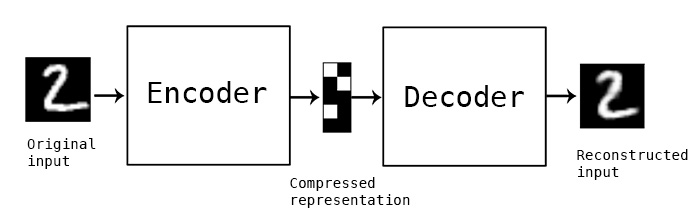
\includegraphics[width=0.8\linewidth]{img/autoencoder_schema.jpg}
	\caption{Struttura di un generico AutoEncoder, da \cite{keras_blog}}
	\label{fig:1.12}
\end{figure}
Il processo di \textit{autoencoding} indica il risultato di un algoritmo di compressione, dove le funzioni di compressione e decompressione presentano le seguenti caratteristiche: sono specifiche dei dati, presentano perdite e sono apprese automaticamente attraverso gli esempi, piuttosto che codificate a mano da un programmatore. L'ultima di queste caratteristiche rimanda immediatamente all'uso di una rete neurale, che infatti è l'implementazione tipica di un autoencoder.

A differenza degli algoritmi di compressione genericamente utilizzati, ad esempio MPEG-2 Audio Layer III (comunemente detto MP3) per l'audio, che si prestano ad un utilizzo ampio, un autoencoder è limitato dal dataset su cui viene addestrato. Le prestazioni su un autoencoder addestrato su di un certo suono o su fotografie di volti crollerebbero drasticamente, su suoni diversi o su fotografie di alberi. Allo stesso modo di alcuni degli algoritmi più comuni, l'output dopo la decompressione presenta una diminuzione di qualità rispetto all'input originale. In compenso è facile addestrare istanze specifiche dell'algoritmo, che presentino buoni risultati su un particolare input, in quanto non sono generalmente necessari nuovi interventi di ingegneria del software ma solo dati appropriati.

Per assemblare un autoencoder sono necessarie tre componenti fondamentali: una funzione che operi la codifica, una che operi la decodifica e una che misuri la distanza che occorre fra la rappresentazione compressa e quella ottenuta dalla ricostruzione, in termini di perdita di dati (ovvero una loss function).
Decoder ed encoder (fig \ref{fig:1.12}) sono tipicamente funzioni parametriche (reti neurali), differenziabili rispetto alla funzione di distanza in modo da essere ottimizzabili per minimizzare la perdita in ricostruzione, usando lo \textit{Stochastic Gradient Descent} (SGD).
\section{Modelli Generativi} % (fold)
\label{sec:modelli_generativi}
All'inizio di questo elaborato è stato citato brevemente il concetto di \textit{modello generativo}, poi ripreso in alcuni esempi nella sezione riguardante le reti ricorrenti.

Gli algoritmi finora elencati, nella loro implementazione più semplice, formano modelli che tipicamente stabiliscono i confini che intercorrono fra le varie classi a cui possono appartenere i dati in input. Per questa ragione sono detti \textit{modelli discriminativi}, in quanto non si preoccupano di fare assunzioni sull'origine dei dati forniti ma si limitano a categorizzarli nel modo più efficace. Lo scopo di un modello generativo, invece, è quello di apprendere come sono stati generati i dati ottenuti, producendo una rappresentazione delle classi a cui appartengono attraverso l'analisi delle caratteristiche rilevate nell'input.

Da un punto di vista matematico, un modello discriminativo cerca di apprendere la distribuzione di probabilità condizionata rispetto ai dati, in formule: 
\begin{equation}
	\label{conditional}
	f(\boldsymbol{x}) = arg \max_y p(\boldsymbol{y}|\boldsymbol{x})
\end{equation}
Per contro, un modello generativo cerca di apprendere la distribuzione di probabilità congiunta, ovvero, usando la regola di Bayes (e liberandoci di $p(x)$, in quanto si massimizza secondo $y$):
\begin{equation}
	\label{joint}
	f(\boldsymbol{x}) = arg\max_y p(\boldsymbol{y}|\boldsymbol{x})p(\boldsymbol{y})
\end{equation}
che corrisponde a $p(x, y)$. Come si può notare intuitivamente, ad un modello generativo è richiesta una complessità superiore che si può tradurre in un calo di prestazioni su compiti meno elaborati, rispetto ai modelli discriminativi, ad esempio nella classificazione. D'altra parte un modello discriminativo non è in grado di cogliere caratteristiche e relazioni complesse fra i dati in input e le variabili target, né è in grado di produrre dati originali analoghi a quelli appresi, proprietà che rendono preferibile un modello generativo per compiti di apprendimento non supervisionato e che sono fondamentali per generare astrazioni come quelle ricercate nella riproduzione di disegni a mano.
% section modelli_generativi (end)
\section{Variabili latenti} % (fold)
\label{sec:variabili_latenti}
Una variabile latente è una variabile casuale che condiziona la generazione dell'output di un modello. Volendo generare immagini di cifre scritte a mano (database MNIST), se nella metà sinistra della cifra è presente metà del carattere \textit{5}, non si può accettare che nella metà destra compaia metà del carattere \textit{0}. In questo caso, la variabile latente permette di stabilire in precedenza quale carattere generare prima di assegnare valori ai pixel. La variabile è detta \textit{latente} poiché, dato il carattere prodotto dal modello, non si possiede necessariamente l'informazione riguardante quale assetto della variabile l'abbia generato.

Prima di poter dire che un modello è in grado di rappresentare il dataset considerato per ogni punto $\boldsymbol{x}$, ci si deve assicurare che esista un assetto della variabile latente che permette al modello di generare un punto molto simile ad esso. Formalmente si supponga di avere un vettore di variabili latenti $\boldsymbol{z}$, in uno spazio multidimensionale $\boldsymbol{Z}$ che si può facilmente campionare in accordo ad una qualche funzione di densità di probabilità (PDF - Probability Density Function) $P(\boldsymbol{z})$ definita su $\boldsymbol{Z}$. Successivamente, si supponga di avere una famiglia di funzioni deterministiche $f(\boldsymbol{z}, \boldsymbol{\theta)}$, parametrizzate rispetto ad un vettore $\boldsymbol{\theta}$ su di un qualche spazio $\boldsymbol{\Theta}$, dove $f : \boldsymbol{Z} x \boldsymbol{\Theta} \rightarrow \boldsymbol{\chi}$. $f$ è deterministica ma, se $\boldsymbol{z}$ è casuale e $\boldsymbol{\theta}$ è fissato, allora $f(\boldsymbol{z}; \boldsymbol{\theta})$ è una variabile casuale nello spazio $\boldsymbol{\chi}$. Si desidera ottimizzare $\boldsymbol{\theta}$ in modo da poter campionare $\boldsymbol{z}$ da $P(\boldsymbol{z})$ e, con alta probabilità, $f(\boldsymbol{z}; \boldsymbol{\theta})$ sarà analoga alle $\boldsymbol{x}$ del dataset considerato.

In modo matematicamente rigoroso, si può affermare che l'obbiettivo è massimizzare la probabilità di ogni $\boldsymbol{x}$ nel training set lungo tutto il procedimento generativo, in accordo a:
\begin{equation}
	\label{probability}
	P(\boldsymbol{x}) = \int P(\boldsymbol{x} | \boldsymbol{z}; \boldsymbol{\theta}) P(\boldsymbol{z})d\boldsymbol{z}
\end{equation}

Qui $f(\boldsymbol{z}, \boldsymbol{\theta)}$ è stato rimpiazzato da $P(\boldsymbol{x} | \boldsymbol{z}; \boldsymbol{\theta})$, che permette di rendere esplicita la dipendenza di $\boldsymbol{x}$ da $\boldsymbol{z}$ attraverso la regola delle probabilità totali. L'intuizione dietro a questo framework, detto \textit{"maximum likelihood"}, è che se il modello è in grado di riprodurre esempi del training set, sarà probabilmente in grado di generare esempi analoghi e con poca probabilità produrrà risultati molto diversi.
% section variabili_latenti (end)
\section{Variational Autoencoder}
\label{sec:vae}
\begin{figure}[ht]
	\centering
	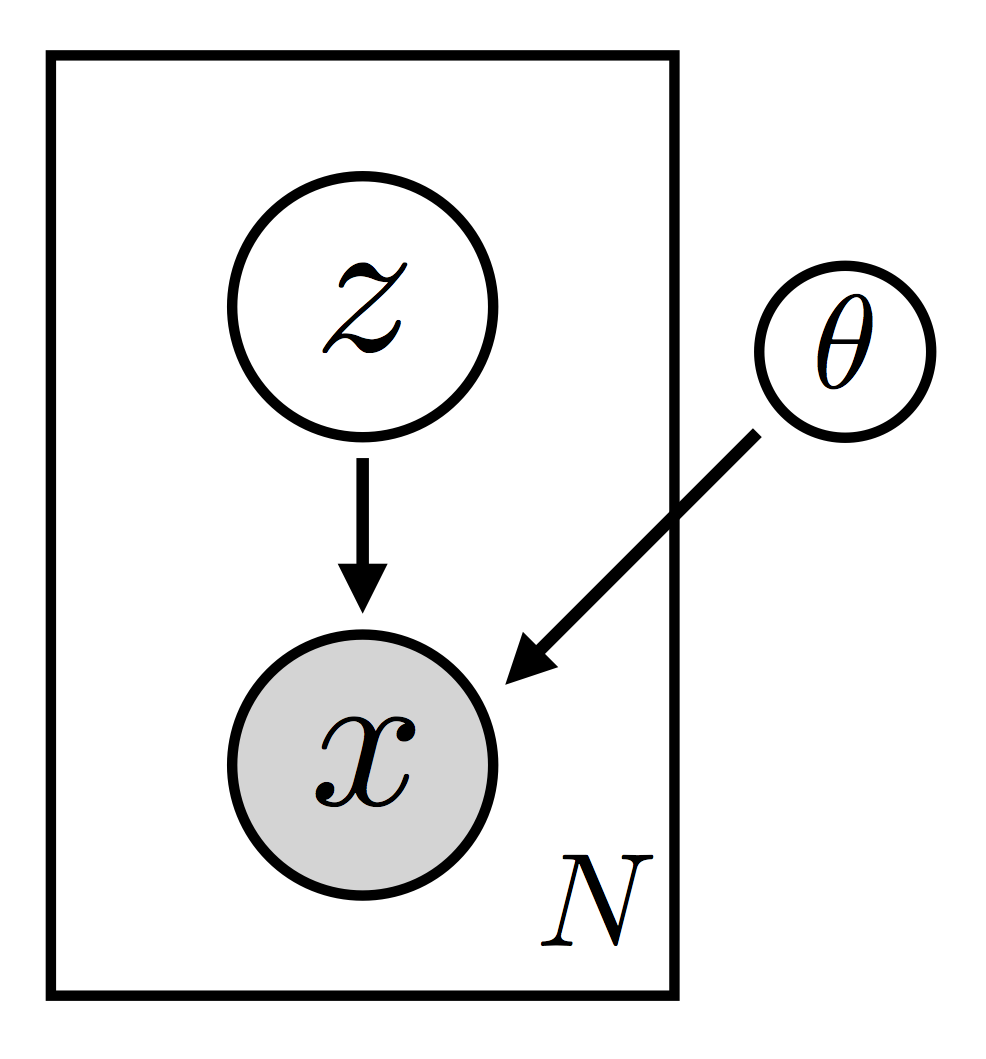
\includegraphics[width=0.4\textwidth]{img/vae_model.png}
	\caption{Modello di un VAE, da \cite{VAE_tut}}
	\label{fig:1.13}
\end{figure}
Seppur fondandosi su principi matematici diversi, i variational autoencoder \cite{VAE} realizzano l'implementazione di un modello generativo attraverso una struttura analoga a quella degli autoencoder tradizionali, a causa della presenza di un encoder ed un decoder nella propria struttura. Si tratta di una classe di modelli che si basa sulla generazione condizionata da una variabile latente.

Nei VAE, la scelta della distribuzione di output è spesso gaussiana, ovvero della forma:
\begin{equation}
	\label{gaussian_probability}
	P(\boldsymbol{x} | \boldsymbol{z}; \boldsymbol{\theta}) = \mathcal{N}(\boldsymbol{x}|f(\boldsymbol{z}; \boldsymbol{\theta}), \sigma^2 * \boldsymbol{I})
\end{equation}
Il che significa che ha media $f(\boldsymbol{z}; \boldsymbol{\theta})$ e covarianza pari alla matrice identità moltiplicata per un qualche scalare $\sigma$ (che è un iperparametro). In ogni caso ciò non è obbligatorio, ad esempio, se $\boldsymbol{x}$ fosse binario, allora $P(\boldsymbol{x} | \boldsymbol{z})$ potrebbe essere una distribuzione di Bernoulli parametrizzata da $f(\boldsymbol{z}; \boldsymbol{\theta})$. La proprietà fondamentale è che $P(\boldsymbol{x} | \boldsymbol{z})$ sia computabile e continua in $\theta$.

La necessità della variabile latente è quella di rappresentare il più accuratamente possibile l'informazione latente. Dovendo ad esempio rappresentare delle cifre scritte a mano (MNIST) dovrebbe non solo determinare quale cifra rappresentare ma anche l'angolo con cui disegnarla, lo spessore del tratto ed altre proprietà prettamente stilistiche. A complicare le cose c'è il fatto che queste proprietà potrebbero presentare dipendenze: una cifra maggiormente inclinata potrebbe essere correlata ad una scrittura più frettolosa e, di conseguenza, ad un tratto più sottile. Idealmente si vorrebbe evitare di stabilire manualmente quali informazioni verranno codificate in ogni dimensione di $\boldsymbol{z}$, inoltre sarebbe da evitare anche la descrizione specifica delle dipendenze fra le dimensioni. L'approccio sfruttato dai VAE è inusuale: partono dall'assunto che non ci sia un'interpretazione semplice delle dimensioni, affermando che campioni di $\boldsymbol{z}$ possano invece essere estratti da una distribuzione semplice, ovvero $\mathcal{N}(0, \boldsymbol{I})$. La chiave di questa logica sta nell'osservare che una distribuzione qualunque in \textit{d} dimensioni, può essere generata attraverso un set di \textit{d} variabili casuali con distribuzione normale, mappante tramite una funzione sufficientemente complicata\footnote{In una dimensione si può utilizzare l'inversa della funzione a distribuzione cumulativa (CDF - cumulative distribution function) della distribuzione desiderata, composta con la CDF di una Gaussiana, in estensione al principio di \textit{"inverse transform sampling"}. Per dimensioni multiple si può applicare il medesimo processo cominciando con la distribuzione marginale di una dimensione e ripetendo con quella condizionale di ogni dimensione aggiuntiva. Si veda "inversion method" e "conditional distribution method" in Devroye et al. \cite{rvg}}. In generale non c'è da porsi il problema di assicurarsi che esista la struttura latente, qualora questa struttura aiuti il modello a riprodurre accuratamente (ovvero, massimizzare la verosimiglianza) i dati del training set allora il modello la imparerà in qualche layer.

Per massimizzare l'equazione \ref{probability}, come genericamente si fa nel machine learning, si cerca una formula computabile per $P(\boldsymbol{x})$, se ne prende il gradiente e con esso si ottimizza il modello tramide SGA (stochastic gradient ascent). Una computazione approssimata di $P(\boldsymbol{x})$ risulta abbastanza semplice: è sufficiente campionare una vasta quantità di valori di $\boldsymbol{z}$, $\{z_1,...,z_n\}$ e calcolare $P(\boldsymbol{x}) \approx \frac{1}{n} \sum_i P(\boldsymbol{x} | z_i)$. Il problema sorge per spazi a molte dimensioni, $n$ potrebbe dover essere estremamente ampio prima di ottenere una stima accurata di $P(\boldsymbol{x})$. La soluzione dei VAE è di evitare la definizione di una misura di somiglianza più accurata che potrebbe essere di difficile implementazione in domini complessi quali le immagini. La scelta ricade piuttosto sull'alterare la procedura di campionamento, per renderla più rapida senza dover modificare la metrica. In sostanza, l'idea è di definire una nuova funzione $Q(\boldsymbol{z} | \boldsymbol{x})$ che cerca di campionare valori di $\boldsymbol{z}$ che potrebbero aver prodotto $\boldsymbol{x}$. La speranza è che lo spazio generato da $Q$ sia minore dello spazio di ogni $\boldsymbol{z}$ che sottostà a $P(\boldsymbol{z})$. Ciò permette di calcolare facilmente $E_{\boldsymbol{z}\sim Q} P(\boldsymbol{x} | \boldsymbol{z})$ a patto che questa sia legata a $P(\boldsymbol{x})$.

Per integrare questo concetto all'interno della computazione della rete neurale, potendo quindi effettuare SGD su tutti i passaggi, altrimenti non differenziabili, si compie un'operazione detta \textit{reparametrization trick}. Si sceglie la funzione di codifica come $Q(\boldsymbol{z} | \boldsymbol{x}) = \mathcal{N}(\boldsymbol{z} | \boldsymbol{\mu}(\boldsymbol{x}; \Theta), \sigma(\boldsymbol{x}; \Theta))$, dove $\mu$ e $\hat\sigma$ sono funzioni deterministiche arbitrarie (ovvero implementabili con una rete neurale) con parametro $\Theta$ che può essere appreso dai dati. Ciò permette di definire una loss function per la rete neurale che non è altro che la somma fra l'errore di ricostruzione nel riprodurre i dati a partire dalla variabile latente $\boldsymbol{z}$ e la \textit{KL divergence} (divergenza di Kullback - Leibler) fra $Q(\boldsymbol{z} | \boldsymbol{x})$ e $P(\boldsymbol{z})$:
\begin{equation}
	\label{vae_loss}
	l = -E_{\boldsymbol{z}\sim Q}[\log(P(\boldsymbol{x} | \boldsymbol{z}))] + KL(Q(\boldsymbol{z} | \boldsymbol{x}) || P(\boldsymbol{z}))
\end{equation}
\begin{figure}[ht]
	\centering
	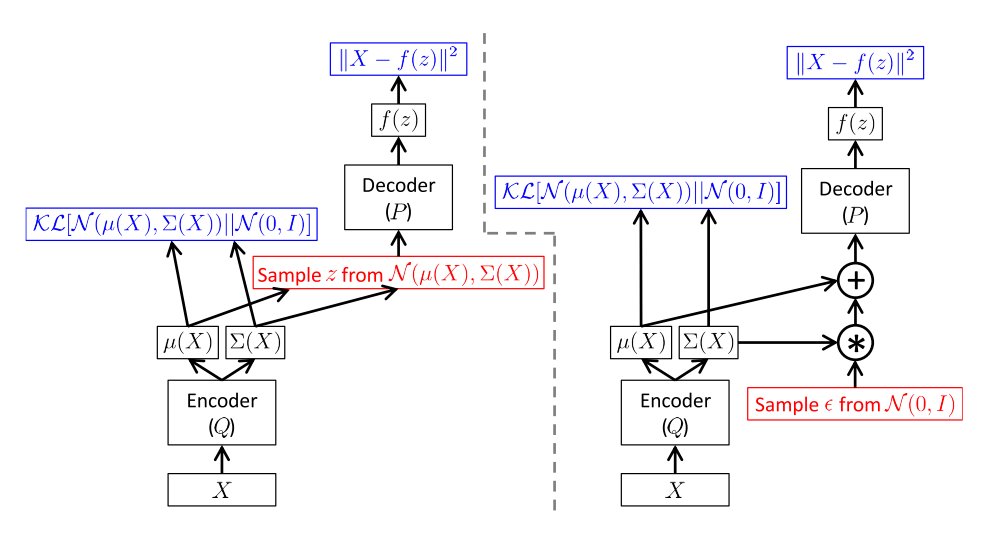
\includegraphics[width=\textwidth]{img/vae_struct.png}
	\caption{Un VAE per intero, a sinistra senza il "reparametrization trick", a destra con. In rosso le operazioni non differenziabili, in blu le loss. Queste due varianti differiscono per il fatto che la retropropagazione si può applicare solo sulla rete a destra.}
	\label{fig:1.14}
\end{figure}

\section{Problemi inversi} % (fold)
\label{sec:problemi_inversi}
Molte applicazioni potenziali delle reti neurali ricadono nella categoria dei problemi inversi. Alcuni esempi includono il controllo di impianti industriali, l'analisi di dati spettrali, le ricostruzioni tomografiche e la cinematica dei robot. Per ogni problema inverso esiste un ben definito problema \textit{diretto} caratterizzato da una mappatura funzionale (ovvero a valore singolo). Di solito ciò corrisponde alla causalità nei sistemi fisici. 

Si consideri un semplice esempio di un problema inverso che riguarda la mappatura fra una variabile unitaria in input e una in output, rispettivamente $t$ e $x$, definito da:
\begin{equation}
	\label{direct}
	x = t + 0.3 \sin(2 \pi t) + \epsilon
\end{equation}
dove $\epsilon$ è una variabile casuale con distribuzione uniforme nell'intervallo (-0.1, 0.1). La mappatura da $t$ a $x$ costituisce un esempio di problema diretto. In assenza del termine di disturbo $\epsilon$, questa mappatura è a valore singolo, ovvero ogni valore di $t$ dà origine ad un singolo valore di $x$. In fig. \ref{fig:1.20} si può notare un dataset di mille punti generati dal campionamento\ref{direct} ad intervalli uguali di $t$ nel raggio (0.0, 1.0). Allo stesso modo viene mostrata la mappatura rappresentata da un MLP standard addestrato su questo dataset. La rete prende un valore in input, possiede cinque unità con funzione d'attivazione \textit{tanh} (tangente iperbolica) e restituisce un output lineare. L'addestramento è stato eseguito con mille cicli completi dell'algoritmo quasi-Newtoniano BFGS \cite{bfgs}. Si può notare che la rete, che approssima la media condizionale dei dati target, dà un'ottima rappresentazione della distribuzione alla base dei dati. Questo risultato è indipendente dalla scelta della struttura della rete, dal valore iniziale dei pesi e dai dettagli della procedura di training.
\begin{figure}[ht]
	\centering
	\includegraphics[width=0.4\textwidth]{img/direct.png}
	\caption{Un semplice esempio di problema diretto: sono evidenziati 1000 punti corrispondenti ai dati (i cerchi) generati dalla mappatura $x = t + 0.3 \sin(2 \pi t) + \epsilon$ dove $\epsilon$ è una variabile casuale. La curva rappresenta il risultato dell'addestramento di un MLP con cinque unità e somma di quadrati come funzione d'errore. La rete approssima la media condizionale del target, che dà una buona rappresentazione del generatore dei dati.}
	\label{fig:1.20}
\end{figure}

Si consideri adesso il corrispondente problema inverso, dove verrà utilizzato lo stesso dataset ma sarà tentata la mappatura dalla variabile $x$ alla variabile $t$. Il risultato dell'addestramento di un'analoga rete neurale è mostrato in fig. \ref{fig:1.21}.
\begin{figure}[ht]
	\centering
	\includegraphics[width=0.4\textwidth]{img/inverse.png}
	\caption{Quest'immagine mostra esattamente lo stesso dataset della figura \ref{fig:1.20}, invertendo input e variabili target. La curva mostra nuovamente il risultato dell'addestramento di una MLP con funzione \textit{sum-of-squares}. Stavolta la rete ottiene un pessimo risultato, continuando a tentare di rappresentare la media condizionale.}
	\label{fig:1.21}
\end{figure}

Di nuovo, la rete tenta di approssimare la media condizionale dei dati di target, ma stavolta ottiene una rappresentazione inadeguata del procedimento che ha generato i dati. La modalità di mappatura della rete adesso è molto più sensibile alla struttura, all'inizializzazione dei pesi, ecc... di quanto non fosse nel caso del problema diretto. Il risultato ottenuto in figura è il migliore che sia stato possibile ricavare dopo attenta ottimizzazione (ovvero la generica soluzione trovata è stata spesso di qualità inferiore a questa). La rete di questo esempio è composta da venti unità ed è stata addestrata per mille cicli col medesimo algoritmo. Evidentemente una MLP convenzionale, addestrata con la somma di quadrati come funzione d'errore, non è in grado di dare una buona rappresentazione della distribuzione di questi dati.
% section problemi_inversi (end)
\section{Mixture Density Network} % (fold)
\label{sec:mdn}
Come spiegato da Bishop \cite{gmm}, se si assume che la distribuzione di probabilità condizionata dei dati di target sia Gaussiana, si può derivare la tecnica dei minimi quadrati utilizzando la massima verosimiglianza. Questo motiva l'idea di rimpiazzare la distribuzione Gaussiana nella densità condizionale del vettore target con un \textit{mixture model} (modello a mistura) \cite{mixture}, che ha la flessibilità per modellare completamente funzioni di distribuzione generiche. La densità di probabilità dei dati target è quindi rappresentata come combinazione lineare di funzioni kernel della forma:
\begin{equation}
	\label{density}
	p(\boldsymbol{x} | \boldsymbol{y}) = \sum\_{i=1}^m \alpha_i(\boldsymbol{x}\phi_i(\boldsymbol{y} | \boldsymbol{X}))
\end{equation}
Dove \textit{m} è il numero di componenti nella mistura e $\alpha_i(\boldsymbol{x})$ sono detti \textit{mixing coefficients} (coefficienti di mescolamento).

Sempre in accordo a Bishop, le funzioni della mistura saranno Gaussiane della forma:
\begin{equation}
	\label{kernel}
	\phi_i(\boldsymbol{y} | \boldsymbol{x}) = \frac{1}{(2\pi)^{\frac{c}{2}}\sigma_i(\boldsymbol{x})^c} \exp\bigg\{-\frac{||\boldsymbol{y} - \boldsymbol{\mu}_i(\boldsymbol{x}||^2}{2\sigma_i(\boldsymbol{x})^2}\bigg\}
\end{equation}
dove $\boldsymbol{\mu}_i$ rappresenta il centro dell'i-esima funzione. L'autore assume che le componenti del vettore di output sono statisticamente indipendenti rispetto ad ogni componente della distribuzione e possono essere descritte dalla varianza $\sigma_i(\boldsymbol{x})$. Questa assunzione può essere rilassata introducendo matrici complete di covarianza per ogni Gaussiana, al costo di un formalismo più complesso. In linea di principio, tuttavia, questa complicazione non è necessaria poiché un \textit{Gaussian Mixture Model} (modello a mistura gaussiana), con componenti date da \ref{kernel}, può approssimare qualunque funzione di densità di probabilità data con precisione arbitraria, a patto di selezionare adeguatamente i coefficienti di mistura e i parametri delle Gaussiane (media e varianza)\footnote{Ottenuti tramite le variabili addestrabili della rete neurale sottostante.}. Di conseguenza la rappresentazione data da \ref{density} e \ref{kernel} è completamente generale e, in particolare, non assume necessariamente che le componenti di $\boldsymbol{t}$ siano statisticamente indipendenti\footnote{Al contrario alla rappresentazione con singola Gaussiana.}.
\begin{figure}[ht]
	\centering
	\includegraphics[width=\textwidth]{img/mdn.png}
	\caption{Rappresentazione di una MDN. L'output della rete neurale determina i parametri di una mistura. Di conseguenza, il modello rappresenta la funzione di densità di probabilità condizionale delle variabili target condizionate all'input $\boldsymbol{x}$ della rete. Immagine da \cite{MDN}}
	\label{fig:1.22}
\end{figure}

Come si può vedere in fig. \ref{fig:1.22}, dato un vettore di input $\boldsymbol{x}$, la MDN fornisce un formalismo generale per modellare una funzione di densità di probabilità condizionata $p(\boldsymbol{y} | \boldsymbol{x})$. Questa combinazione fra reti neurali tradizionali e modelli a mistura è resa possibile utilizzando la verosimiglianza logaritmica della combinazione lineare fra le distribuzioni Gaussiane come funzione di loss per la rete.

Assemblare una MDN incrementa il numero di elementi di output della rete neurale di partenza: dati \textit{c} parametri, con la MDN questi salgono a $(c + 2) * m$, dove \textit{m} è il numero di misture del modello.

Bishop suggerisce alcune restrizioni che i parametri della rete devono soddisfare:
\begin{itemize}
	\item Come richiesto per le probabilità, è necessario che i coefficienti di mistura $\alpha_i$ soddisfino il vincolo $\sum_{i=1}^m = 1$. Per ottenere questa restrizione, in linea di principio, è sufficiente una funzione di attivazione \textit{softmax} per il nodo corrispondente ad $\alpha_i$.
	\begin{equation}
		\label{softmax}
		\alpha_i = \frac{\exp(z_i^\alpha)}{\sum_{j=1}^m\exp(z_j^\alpha)}
	\end{equation}
	dove $z_i^\alpha$ rappresenta l'output corrispondente. Questa restrizione assicura che le quantità $\alpha_i$ siano comprese in (0, 1) e sommino ad uno.
	\item Le varianze $\sigma_i$ rappresentano parametri di scala, di conseguenza è conveniente rappresentarle in termini dell'esponenziale dell'output corrispondente
	\begin{equation}
		\label{exponential}
		\sigma_i = \exp(z_i^\sigma)
	\end{equation}
	che, in un framework Bayesiano, corrisponderebbe alla scelta di una distribuzione a priori non informativa, assumendo che l'output corrispondente $z_i^\sigma$ abbia una distribuzione di probabilità uniforme. Questa rappresentazione ha il beneficio addizionale di evitare configurazioni "patologiche" in cui una o più varianze vanno a zero.
	\item I parametri centrali $\mu_i$ rappresentano parametri di posizione, prendendo in considerazione l'idea che la distribuzione a priori sia non informativa, è conveniente rappresentare direttamente questi parametri dagli output della rete, ovvero:
	\begin{equation}
		\label{mus}
		\mu\_{i,k} = z_{i,k}^\mu
	\end{equation}
\end{itemize}

A questo punto è possibile costruire una funzione di verosimiglianza usando la densità condizionale del vettore di target completo. Dopodiché, per definire una funzione di errore (da usare come loss per la rete), si può utilizzare l'approccio standard del metodo di massima verosimiglianza, che richiede la massimizzazione della funzione di verosimiglianza logaritmica o, equivalentemente, la minimizzazione del logaritmo negativo della verosimiglianza. Di conseguenza, la funzione di errore per una MDN è:
\begin{equation}
	\label{mdnerror}
	\log\mathbb{L}(\boldsymbol{y} | \boldsymbol{x}) = - \log(p(\boldsymbol{y} | \boldsymbol{x})) = - \log\bigg(\sum_{i=0}^m \alpha_i(\boldsymbol{x})\phi_i(\boldsymbol{y} | \boldsymbol{x})\bigg)
\end{equation}
% section mdn (end)
\myChapter{Strumenti}
\section{Librerie software}
\subsection{Keras}
\subsection{Recurrentshop}
\section{Dataset}
\myChapter{Esperimenti}
\section{Introduzione} % (fold)
\label{sec:introduzione}
In questo elaborato si è scelto di riprodurre ed analizzare i risultati presentati da Ha e Eck attraverso tre esperimenti: nel primo è stata scelta la configurazione standard del modello, con un VAE completo e layer LSTM sia nell'encoder che nel decoder, la rete è stata addestrata su due dataset: \textit{cat.npz} (gatti) e \textit{flying\_saucer.npz} (dischi volanti). Nel secondo è stata scelta la configurazione con il solo decoder, utilizzato come modello autoregressivo non condizionato ad una variabile latente (con i pesi inizializzati a zero), in questo caso il layer utilizzato è HyperLSTM\footnote{Questo layer non è stato approfondito nell'introduzione di questo elaborato, si rimanda a \cite{hyperlstm} per ulteriori informazioni.}, che eccelle nella generazione di sequenze, il dataset è stato addestrato sul solo dataset \textit{owl.npz} (gufi), infine è stato addestrato un modello con \textit{Layer Normalization} nell'encoder e HyperLSTM nel decoder\footnote{Soluzione suggerita in \url{https://github.com/tensorflow/magenta/tree/master/magenta/models/sketch_rnn}}, per poter gestire un ampio training set composto da tre categorie: \textit{elephant} (elefanti), \textit{hat} (cappelli) e \textit{snake} serpenti\footnote{In omaggio a \cite{petitprince}}. Di seguito verranno illustrate e confrontate le reti neurali prodotte da queste configurazioni, inoltre verranno mostrate alcune immagini generate tramite diversi approcci che mostreranno la capacità del modello di concettualizzare le proprietà di un disegno.

\begin{minipage}{\linewidth}
\begin{lstlisting}[language = Python, frame = single, caption = {Iperparametri standard di sketch-rnn}, label = {iperparametri}, captionpos = b, basicstyle=\scriptsize]
num_steps=10000000,            # Total number of training set. Keep large.
save_every=500,                # Number of batches per checkpoint creation.
dec_rnn_size=512,              # Size of decoder.
dec_model='lstm',              # Decoder: lstm, layer_norm or hyper.
enc_rnn_size=256,              # Size of encoder.
enc_model='lstm',              # Encoder: lstm, layer_norm or hyper.
z_size=128,                    # Size of latent vector z. Rec. 32, 64 or 128.
kl_weight=0.5,                 # KL weight of loss. Recommend 0.5 or 1.0.
kl_weight_start=0.01,          # KL start weight when annealing.
kl_tolerance=0.2,              # Level of KL loss at which to stop optimizing
batch_size=100,                # Minibatch size. Recommend leaving at 100.
grad_clip=1.0,                 # Gradient clipping. Recommend leaving at 1.0.
num_mixture=20,                # Number of mixtures in Gaussian mixture model.
learning_rate=0.001,           # Learning rate.
decay_rate=0.9999,             # Learning rate decay per minibatch.
kl_decay_rate=0.99995,         # KL annealing decay rate per minibatch.
min_learning_rate=0.00001,     # Minimum learning rate.
use_recurrent_dropout=True,    # Recurrent Dropout without Memory Loss.
recurrent_dropout_prob=0.90,   # Probability of recurrent dropout keep.
use_input_dropout=False,       # Input dropout. Recommend leaving False.
input_dropout_prob=0.90,       # Probability of input dropout keep.
use_output_dropout=False,      # Output droput. Recommend leaving False.
output_dropout_prob=0.90,      # Probability of output dropout keep.
random_scale_factor=0.15,      # Random scaling data augmention proportion.
augment_stroke_prob=0.10,      # Point dropping augmentation proportion.
conditional=True,              # If False, use decoder-only model.
\end{lstlisting}
\end{minipage}
In questa sezione di codice sono mostrati gli iperparametri del modello, coi loro valori di default. Si può notare che \textit{N\textsubscript{z}} = 128 e che decoder e encoder sono simmetrici\footnote{Si ricordi che l'encoder è un layer bidirezionale, di conseguenza la dimensione dello stato finale, dopo la concatenazione, risulta essere 512.}. A partire da questi valori, viene assemblata la rete neurale mostrata in tabella \ref{tab:1}.
\begin{table}[ht]
	\centering
	\begin{tabular}{ccc}
		\hline
		\hline
		Layer & Output shape & Variabili addestrabili \\
		\hline
		\hline
		Input & (?, 250, 5) & 0 \\
		\hline
		Forward LSTM & (?, 256) & 268288 \\
		\hline
		Backward LSTM & (?, 256) & 268288 \\
		\hline
		Mu & (?, 128) & 65664 \\
		\hline
		Log Sigma & (?, 128) & 65664 \\
		\hline
		State initializer & (?, 1024) & 132096 \\
		\hline
		Decoder LSTM & (?, 512) & 1323008 \\
		\hline
		Output & (?, 123) & 63099 \\
		\hline
		\hline
		\multicolumn{3}{c}{Numero di variabili totale: 2186107} \\
		\hline
		\hline
	\end{tabular}
	\caption{I layer ottenuti attraverso la configurazione standard.}
	\label{tab:2}
\end{table}

Nel caso della seconda rete la dimensione del layer ricorrente è sempre 512 ma, per la maggior complessità dei parametri interni, si ottiene una rete com 2218363 variabili addestrabili. L'ultimo modello, infine, presenta 24515195 variabili addestrabili con la dimensione dell'output del decoder pari a 2048 e quella dell'encoder pari a 512 (1024)\footnote{Si omette la tabella, riportando solo le dimensioni fondamentali, per la complessità di lettura derivante dalla struttura dell'HyperLSTM.}.

Con queste reti sono stati condotti vari esperimenti, in particolare: nei modelli condizionali sono state svolte interpolazioni nello spazio di latenza, sia all'interno di una singola classe sia fra classi diverse, inoltre è stato osservato l'esito della variazione del parametro di temperatura sia su interpolazioni che su generazioni condizionali semplici ed in special modo nel modello autoregressivo, sul quale ha un impatto rilevante.
Di seguito i test effettuati saranno illustrati in dettaglio e commentati.
\section{Generazione condizionale} % (fold)
\label{sec:generazione_condizionale}
In questa sezione vengono valutati i disegni ricostruiti \textit{S'}, dato in input un disegno \textit{S}, da parte dei due VAE.
\begin{figure}[ht]
	\centering
	\begin{tabular}{cccc}
		\fbox{\includegraphics[width=0.2\linewidth]{img/cat_enc.png}} &
		\includegraphics[width=0.2\linewidth]{img/cat_dec_0.png} &
		\includegraphics[width=0.2\linewidth]{img/cat_dec_2.png} &
		\includegraphics[width=0.2\linewidth]{img/cat_dec_3.png} \\
		\includegraphics[width=0.2\linewidth]{img/cat_dec_4.png} &
		\includegraphics[width=0.2\linewidth]{img/cat_dec_5.png} &
		\includegraphics[width=0.2\linewidth]{img/cat_dec_6.png} &
		\includegraphics[width=0.2\linewidth]{img/cat_dec_7.png}
	\end{tabular}
	\caption{La prima immagine è estratta dal dataset, le altre sono immagini originali generate dal modello standard}
	\label{fig:1.17}
\end{figure}
Questo primo esempio \ref{fig:1.17} illustra un risultato semplice, quanto interessante: la figura nel riquadro è stata passata come input alla prima rete neurale, le successive sono immagini generate dalla rete attraverso un parametro di temperatura di 0.8, condizionate allo stesso input. L'ampiezza del parametro di temperatura permette alla rete una maggiore libertà \ref{sec:modello}, aumentando la varianza sull'offset dei punti\footnote{Al prezzo di immagini maggiormente confuse.}, il che mostra le potenzialità del modello nel creare sketch simili ma unici ed originali, a partire da un singolo input.

Il modello è anche in grado di reinterpretare un disegno proveniente da una classe qualunque, secondo le caratteristiche su cui è stato addestrato. Se infatti alla rete viene chiesto di riprodurre dati da una classe che non conosce, questa produrrà sketch che combineranno proprietà dovute al condizionamento con le proprietà dovute all'apprendimento, talvolta aggiungendo dettagli, talvolta distorcendo le strutture date.
\subsection{Variazioni di temperatura} % (fold)
\label{sub:variazioni_di_temperatura}
Come detto in precedenza \ref{sec:modello}, nell'operazione di campionamento di un disegno viene introdotto un parametro $\tau$ il cui scopo è contenere la variabilità dell'offset e dei parametri categorici. La variazione di questo parametro, generando schizzi condizionati dallo stesso disegno di partenza, porta ad output che vanno da una riproduzione più fedele dell'input ad una più fantasiosa.

Anche in questo caso è interessante osservare come ciò si rifletta sui tentativi della rete di interpretare oggetti sconosciuti secondo le proprie categorie. Di fatto in questa situazione il parametro di temperatura diventa il peso assegnato alle nuove caratteristiche osservate, con un parametro più basso che obbliga il VAE ad attenersi il più possibile alle proprietà dell'input.
% subsection variazioni_di_temperatura (end)
\subsection{Interpolazioni} % (fold)
\label{sub:interpolazioni}
Interpolando fra vettori latenti è possibile visualizzare come un'immagine muta in un'altra, osservando la ricostruzione dell'interpolazione. Considerato che sullo spazio di latenza viene forzata una Gaussiana come distribuzione a priori, è lecito aspettarsi una mutazione più fluida e priva di "salti" nello spazio fra due vettori di latenza diversi. Un modello addestrato col parametro del peso della divergenza KL ($w_KL$ \ref{sub:training}) posto ad un valore alto dovrebbe produrre immagini più aderenti ai dati, dato un vettore di latenza $\boldsymbol{z}$ interpolato sfericamente, rispetto ad una rete addestrata con un valore di $w_KL$ più basso.

Per dimostrare questo risultato è sufficiente addestrare diversi modelli sugli stessi dataset, utilizzando valori diversi di $w_KL$. Si riporta l'esperimento svolto da Ha e Eck sui dataset \textit{cat} e \textit{pigs}.
% subsection interpolazioni (end)
\subsection{Analogie fra disegni} % (fold)
\label{sub:analogie_fra_disegni}
L'esempio di interpolazione in fig. suggerisce che il vettore di latenza $\boldsymbol{z}$ codifichi caratteristiche concettuali di un disegno. Modelli addestrati con un minor peso alla divergenza KL, sono in grado di incrementare i dettagli di uno sketch con caratteristiche prese da un altro, ad esempio aggiungendo un corpo ad una testa di gatto, acquisendolo dal disegno di un maiale. Questo è possibile perché lo spazio di latenza è abbastanza "rilassato" da permettere che ogni vettore interpolato fra due vettori di latenza risulti in un disegno coerente, ciò permette di eseguire operazioni aritmetiche fra vettori ottenuti da diversi disegni ed esplorare come il modello organizzi lo spazio latente per rappresentare i concetti nella moltitudine degli sketch generati.

Nello specifico della figura: è stato sottratto il vettore latente codificante la testa di un maiale da quello che codifica un maiale intero, ciò ha portato ad un vettore contenente le caratteristiche di un corpo. Aggiungendo questa differenza al vettore che rappresenta la testa di un gatto è stato ottenuto un gatto completo. Allo stesso modo è stato rimosso il corpo di un maiale ottenendo prima la codifica tramite gatti.
% subsection analogie_fra_disegni (end)
% section generazione_condizionale (end)
\section{Generazione non condizionale} % (fold)
\label{sec:generazione_non_condizionale}
Come caso particolare, è possibile addestrare il modello per generare disegni non condizionati ad un input, è il caso della terza rete che è stata assemblata per gli esperimenti di questo elaborato. Rimuovendo l'encoder si ottiene un modello autoregressivo privo di variabile latente, di conseguenza gli stati iniziali e delle celle vengono inizializzati a zero. Gli input $x_i$ della RNN ad ogni time step sono solo $s_{i-1}$ o $S{i-1}'$ dato che non c'è nessun vettore da concatenare. Con questa struttura è stata sperimentata la generazione al variare del parametro di temperatura.
\begin{figure}[ht]
	\centering
	\begin{tabular}{c}
		\includegraphics[width=\linewidth]{img/owl_temp_02.png} \\
		\includegraphics[width=\linewidth]{img/owl_temp_04.png} \\
		\includegraphics[width=\linewidth]{img/owl_temp_05.png} \\
		\includegraphics[width=\linewidth]{img/owl_temp_06.png} \\
		\includegraphics[width=\linewidth]{img/owl_temp_08.png} \\
		\includegraphics[width=\linewidth]{img/owl_temp_1.png}
	\end{tabular}
	\caption{Immagini generate dal modello autoregressivo al variare del parametro di temperatura}
\end{figure}

Si può notare come la mancanza di uno spazio di latenza a cui condizionare l'output renda preminente l'impatto della variazione della temperatura sulla variabilità dei disegni generati: al crescere del parametro la rete passa da disegni estremamente fedeli ed accurati a disegni molto più vaghi ed imprecisi.

\subsection{Predire il finale di un disegno incompleto} % (fold)
\label{sub:predire_il_finale_di_un_disegno_incompleto}
Un'interessante applicazione pratica della variante con il solo decoder è che rende possibile utilizzare \texttt{sketch-rnn} per offrire spunti artistici, completando sketch in input. Il layer ricorrente della rete viene utilizzato in un primo momento per generare una codifica della porzione di disegno ricevuta in input, ottenendo un hidden state condizionato ad esso. Successivamente lo stato generato viene utilizzato per inizializzare nuovamente la rete, che proseguirà l'esecuzione fino in fondo, completando la sequenza a partire da quella data.
% subsection predire_il_finale_di_un_disegno_incompleto (end)
% section generazione_non_condizionale (end)

\begin{minipage}{\linewidth}
\begin{lstlisting}[language = Python, frame = single, caption = {}, captionpos = b]

\end{lstlisting}
\end{minipage}
\myChapter{Conclusioni}
% \chapter{esercizi}

\begin{enumerate}
\medskip
\item 
Scrivere le possibili evoluzioni del programma 
\begin{verbatim}
                       		co X: = X+2 // X: = X+1 oc
\end{verbatim}
assumendo che ciascun assegnamento � realizzato da tre azioni atomiche che
caricano X in un registro (\verb"Load R X"), incrementano il valore del registro (\verb"Add R v") e memorizzano il valore del registro((\verb"Store R X"). Per ciascuna delle esecuzioni risultanti dall�interleaving delle azioni atomiche descrivere il contenuto dopo ogni passo della locazione condivisa X e dei registri privati,  $R_1$ del processo che esegue il primo assegnamento ed  $R_2$  per il processo che esegue il secondo assegnamento. Se assuma che il valore iniziale di X sia 50.
\medskip
\item
Si definisca il problema della \emph{barrier synchronization} e si descrivano per sommi capi i differenti approcci alla sua soluzione. Se ne fornisca quindi una soluzione dettagliata utilizzando i semafori.
\medskip
\item
Considerare n api ed un orso che possono avere accesso ad una tazza di miele
inizialmente  vuota e con una capacit� di k porzioni. L'orso dorme finch� la
tazza � piena di k-porzioni,  quindi mangia tutto il miele e si rimette a
dormire. Le api riforniscono in continuazione la  tazza con una porzione di
miele finch� non si riempie; l'ape che aggiunge la k-esima porzione sveglia
l'orso. Fornire una soluzione al problema modellando orso ed api come  processi
e utilizzando un monitor per gestire le loro operazioni sulla tazza. Prevedere che le api possano eseguire l'operazione \emph{produce-honey} anche concorrentemente.
 \medskip
 \item  Descrivere le primitive di scambio messaggi send e receive sia sincrone che asincrone ed implementare
 \vspace{-0.5cm}
 \begin{verbatim}
       - synch_send(v:int)
       - send(v:int)
       - receive(x:int)
\end{verbatim}
 \vspace{-0.3cm}
utilizzando le primitive di LINDA.

\end{enumerate}

\begin{thebibliography}{99}

\bibitem{sketchrnn}{David Ha, Douglas Eck - \emph{A Neural Representation of 
Sketch Drawings} - 	arXiv:1704.03477, 2017}

\bibitem{quickdraw}{J. Jongejan, H. Rowley, T. Kawashima, J. Kim, and N. 
Fox-Gieg. - \emph{The Quick, Draw! - A.I. Experiment.} - \url{https://quickdraw.withgoogle.com/}, 
2016.}

\bibitem{keras}{Chollet, Fran\c{c}ois and others - \emph{Keras} - GitHub, 
\url{https://github.com/keras-team/keras}}

\bibitem{tensorflow}{Martín Abadi, Ashish Agarwal, Paul Barham, Eugene Brevdo,
Zhifeng Chen, Craig Citro, Greg S. Corrado, Andy Davis,
Jeffrey Dean, Matthieu Devin, Sanjay Ghemawat, Ian Goodfellow,
Andrew Harp, Geoffrey Irving, Michael Isard, Rafal Jozefowicz, Yangqing Jia,
Lukasz Kaiser, Manjunath Kudlur, Josh Levenberg, Dan Mané, Mike Schuster,
Rajat Monga, Sherry Moore, Derek Murray, Chris Olah, Jonathon Shlens,
Benoit Steiner, Ilya Sutskever, Kunal Talwar, Paul Tucker,
Vincent Vanhoucke, Vijay Vasudevan, Fernanda Viégas,
Oriol Vinyals, Pete Warden, Martin Wattenberg, Martin Wicke,
Yuan Yu, and Xiaoqiang Zheng. - \emph{TensorFlow: Large-scale machine 
learning on heterogeneous systems} - \url{tensorflow.org}, 2015}

\bibitem{GAN}{I. Goodfellow. \emph{NIPS 2016 Tutorial: Generative Adversarial 
Networks.} - ArXiv e-prints, Dec. 2017.}

\bibitem{VI}{D. P. Kingma and M. Welling. \emph{Auto-Encoding Variational Bayes.} - 
ArXiv e-prints, Dec. 2013.}

\bibitem{AR}{S. Reed, A. van den Oord, N. Kalchbrenner, S. Gómez Colmenarejo, 
Z. Wang, D. Belov, and N. de Freitas. \emph{Parallel Multiscale Autoregressive 
Density Estimation.} - ArXiv e-prints, Mar. 2017.}

\bibitem{etichetta3}{Dustin Tran and Alp Kucukelbir and Adji B. Dieng and Maja 
Rudolph and Dawen Liang and David M. Blei - \emph{Edward: A library for 
probabilistic modeling, inference, and criticism} - arXiv preprint arXiv:1610.09787,
 2016}



\end{thebibliography}

%--------------------------------------------------------------
\end{document}
%--------------------------------------------------------------
